\documentclass{article} % use larger type; default would be 10pt

\usepackage{tikz}
\usepackage{pgfplots}
\usetikzlibrary{calc}
\usetikzlibrary{arrows}
\usetikzlibrary{patterns}
        \newcommand\degree[0]{^{\circ}}

\title{Play with TikZ}
\author{Just Us}
%\date{} % Activate to display a given date or no date (if empty),
         % otherwise the current date is printed 

\begin{document}
\maketitle

\section{Chapter 8}




ch8-1 sine, cosine, secant, csc, tan, cot

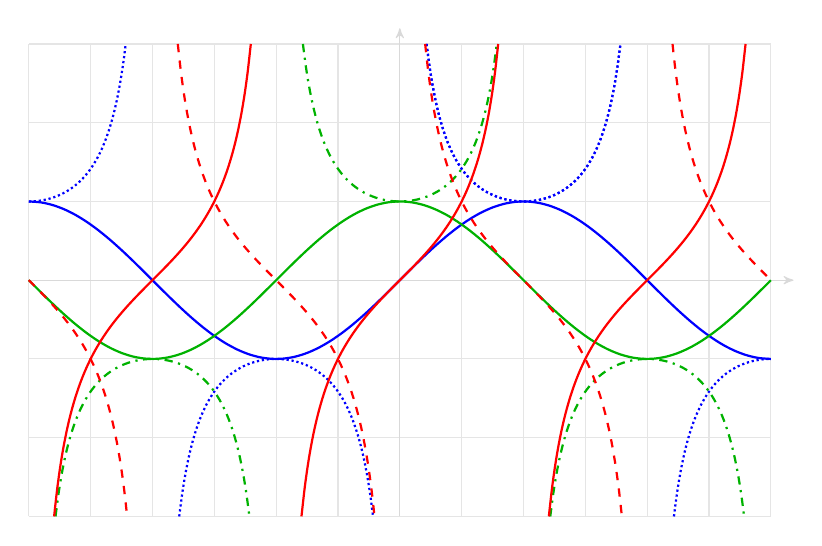
\begin{tikzpicture} 
\draw[gray!20!white] (-3*pi/2,-3) grid[xstep=pi/4, ystep=1] (3*pi/2,3);
\draw[gray!30!white, ->,>=stealth'] (-3*pi/2,0) -- (5.,0);
\draw[gray!30!white, ->,>=stealth'] (0,-3) -- (0,3.2);
\draw[samples=65, domain=-3*pi/2:3*pi/2, variable=\x,smooth, blue, thick] plot (\x,{ sin( deg(\x) });
\def\as{asin(1/3)*pi/180};
\draw[samples=65, domain={\as}:{pi-\as}, variable=\x,smooth, blue, thick, densely dotted] plot (\x,{ cosec( deg(\x) });
\draw[samples=65, domain={-3/2*pi}:{-pi-\as}, variable=\x,smooth, blue, thick, densely dotted] plot (\x,{ cosec( deg(\x) });
\draw[samples=65, domain={-pi+\as}:{-\as}, variable=\x,smooth, blue, thick, densely dotted] plot (\x,{ cosec( deg(\x) });
\draw[samples=65, domain={\as}:{pi-\as}, variable=\x,smooth, blue, thick, densely dotted] plot (\x,{ cosec( deg(\x) });
\draw[samples=65, domain={pi+\as}:{3/2*pi}, variable=\x,smooth, blue, thick, densely dotted] plot (\x,{ cosec( deg(\x) });

\def\ac{acos(1/3)*pi/180};
\draw[samples=65, domain=-3*pi/2:3*pi/2, variable=\x,smooth, green!70!black, thick] plot (\x,{ cos( deg(\x) });
\draw[samples=65, domain={-\ac}:{\ac}, variable=\x,smooth, green!70!black, thick, dashdotted] plot (\x,{ sec( deg(\x) });
\draw[samples=65, domain={-pi-\ac}:{-pi+\ac}, variable=\x,smooth, green!70!black, thick, dashdotted] plot (\x,{ sec( deg(\x) });
\draw[samples=65, domain={pi-\ac}:{pi+\ac}, variable=\x,smooth, green!70!black, thick, dashdotted] plot (\x,{ sec( deg(\x) });

\def\at{atan(3)*pi/180};
\def\att{atan(1/3)*pi/180};
\draw[samples=65, domain={-\at}:{\at}, variable=\x,smooth,red, thick] plot (\x,{ tan( deg(\x) });
\draw[samples=65, domain={pi-\at}:{pi+\at}, variable=\x,smooth,red, thick] plot (\x,{ tan( deg(\x) });
\draw[samples=65, domain={-pi-\at}:{-pi+\at}, variable=\x,smooth,red, thick] plot (\x,{ tan( deg(\x) });
\draw[samples=65, domain={\att}:{pi-\att}, variable=\x,smooth,red, thick, dashed] plot (\x,{ cot( deg(\x) });
\draw[samples=65, domain={-pi+\att}:{-\att}, variable=\x,smooth,red, thick, dashed] plot (\x,{ cot( deg(\x) });
\draw[samples=65, domain={-3/2*pi}:{-pi-\att}, variable=\x,smooth,red, thick, dashed] plot (\x,{ cot( deg(\x) });
\draw[samples=65, domain={pi+\att}:{3/2*pi}, variable=\x,smooth,red, thick, dashed] plot (\x,{ cot( deg(\x) });

\end{tikzpicture}
\newline


fig-8-1-1 three unit circles

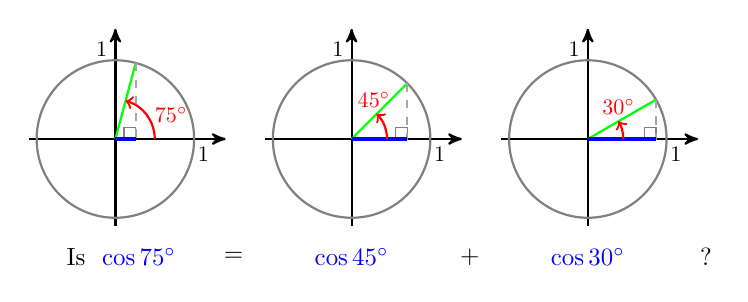
\begin{tikzpicture}
\coordinate (O) at (0,0);
\draw[black,thick,->,>=stealth'] (-1.1,0)--++(2.5,0) node[below left, xshift=-3, scale=.8] {1};
\draw[black,thick,->,>=stealth'] (0,-1.1)--++(0,2.50) node[below left, yshift=-2, scale=.8] {1};
\draw[gray,thick] (O) circle(1cm);
\coordinate (P) at (75:1cm);
\coordinate (Q) at ($ cos(75)*(1,0) $);
\draw[gray] (Q) rectangle ++(-.15,.15);
\draw[green,thick] (P)--(O);
\draw[gray!70!,thick,dashed] (P)--(Q);
\draw[blue, ultra thick] (O)--(Q);
\node[scale=.9] at (-.5,-1.5) {Is};
\node[scale=.9, text=blue] at (.3,-1.5) {$\cos 75\degree$};
\node[scale=.9] at (1.5,-1.5) {$=$};
\draw[red,thick,->] (0.5,0) arc(0:75:0.5) node[right, midway, scale=.8] {$75\degree$};

%second circle
\coordinate (O) at (3,0);
\draw[black,thick,->,>=stealth'] ($ 3*(1,0)+(-1.1,0) $)--++(2.5,0) node[below left, xshift=-3, scale=.8] {1};
\draw[black,thick,->,>=stealth'] ($ 3*(1,0)+(0,-1.1) $)--++(0,2.50) node[below left, yshift=-2, scale=.8] {1};
\draw[gray,thick] (O) circle(1cm);
\coordinate (P) at ($ 3*(1,0)+(45:1cm) $);
\coordinate (Q) at ($ 3*(1,0)+ cos(45)*(1,0) $);
\draw[gray] (Q) rectangle ++(-.15,.15);
\draw[green,thick] (P)--(O);
\draw[gray!70!,thick,dashed] (P)--(Q);
\draw[blue, ultra thick] (O)--(Q);
\node[scale=.9, text=blue] at ($ 3*(1,0)+(0,-1.5) $) {$\cos 45\degree$};
\node[scale=.9] at ($ 3*(1,0)+(1.5,-1.5) $) {$+$};
\draw[red,thick,->] ($ 3*(1,0)+(0.45,0) $) arc(0:45:0.45) node[above, xshift=-1, yshift=2 , inner sep=0,  scale=.8] {$45\degree$};

%third circle
\coordinate (O) at (6,0);
\draw[black,thick,->,>=stealth'] ($ 6*(1,0)+(-1.1,0) $)--++(2.5,0) node[below left, xshift=-3, scale=.8] {1};
\draw[black,thick,->,>=stealth'] ($ 6*(1,0)+(0,-1.1) $)--++(0,2.50) node[below left, yshift=-2, scale=.8] {1};
\draw[gray,thick] (O) circle(1cm);
\coordinate (P) at ($ 6*(1,0)+(30:1cm) $);
\coordinate (Q) at ($ 6*(1,0)+ cos(30)*(1,0) $);
\draw[gray] (Q) rectangle ++(-.15,.15);
\draw[green,thick] (P)--(O);
\draw[gray!70!,thick,dashed] (P)--(Q);
\draw[blue, ultra thick] (O)--(Q);
\node[scale=.9, text=blue] at ($ 6*(1,0)+(0,-1.5) $) {$\cos 30\degree$};
\node[scale=.9] at ($ 6*(1,0)+(1.5,-1.5) $) {?};
\draw[red,thick,->] ($ 6*(1,0)+(0.45,0) $) arc(0:30:0.45) node[above, xshift=0, yshift=2 , inner sep=0,  scale=.8] {$30\degree$};

\end{tikzpicture}
\newline





fig-8-1-2 sine graph
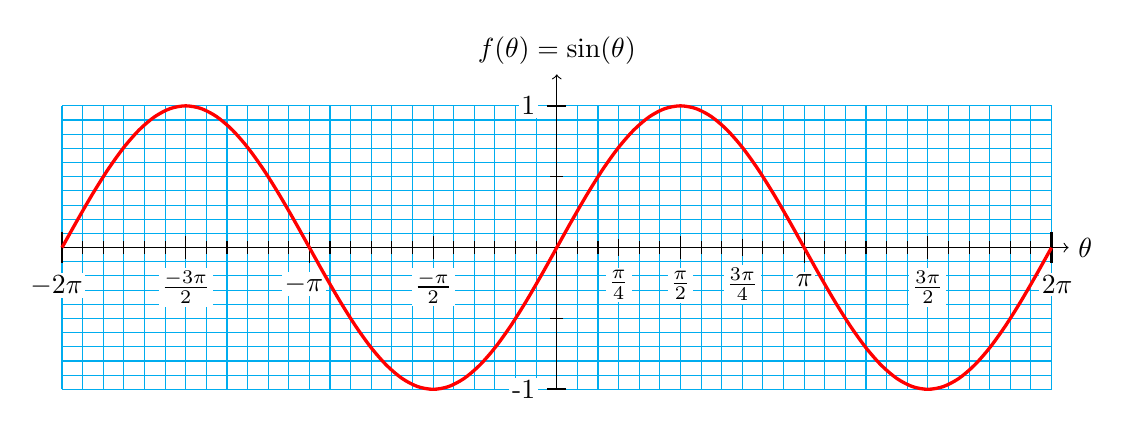
\begin{tikzpicture}
\draw[cyan,xstep=pi/12,ystep=0.18]
(-2*pi,-1.8) grid (2*pi,1.8);

\draw[->] (-6.3,0) -- (6.5,0) node[right] {$\theta$};
\draw[->] (0,-1.8) -- (0,2.2) node[above] {$f(\theta)=\sin(\theta)$};

\foreach \x in {-24,-23,...,24}
\draw[black] ($ pi*\x /12*(1,0) +(0,.08) $) --++(0,-.16);
\foreach \y in {-0.9, 0.9}
\draw[black] (.08,\y ) --++(-.16,0);
\foreach \y in {-1,1}
\draw[black, thick] (.12,1.8*\y ) --++(-.24,0) node[anchor=east, xshift=-3, fill=white, inner sep=1pt] {\y};

\draw[black, thick] (-2*pi,.2) --++(0,-.4) node[anchor=north, xshift=-2,yshift=-3, fill=white, inner sep=1pt] {$-2\pi$};
\draw[black, thick] (2*pi,.2) --++(0,-.4) node[anchor=north, xshift=2,yshift=-3, fill=white, inner sep=1pt] {$2\pi$};

\draw[black] (pi,.2) --++(0,-.4) node[anchor=north, yshift=-3, fill=white, inner sep=1pt] {$\pi$};

\draw[black] (pi,.2) --++(0,-.4) node[anchor=north, yshift=-3, fill=white, inner sep=1pt] {$\pi$};
\draw[black] (-pi,.2) --++(0,-.4) node[anchor=north, xshift=-2,yshift=-3, fill=white, inner sep=1pt] {$-\pi$};
\draw[black] (-pi/2,.15) --++(0,-.3) node[anchor=north, yshift=-3, fill=white, inner sep=1pt] {$\frac{-\pi}{2}$};
\draw[black] (pi/2,.15) --++(0,-.3) node[anchor=north, yshift=-3, fill=white, inner sep=1pt] {$\frac{\pi}{2}$};
\draw[black] (3*pi/2,.15) --++(0,-.3) node[anchor=north, yshift=-3, fill=white, inner sep=1pt] {$\frac{3\pi}{2}$};
\draw[black] (-3*pi/2,.15) --++(0,-.3) node[anchor=north, yshift=-3, fill=white, inner sep=1pt] {$\frac{-3\pi}{2}$};

\draw[black] (pi/4,.11) --++(0,-.22) node[anchor=north, yshift=-4, fill=white, inner sep=1pt] {$\frac{\pi}{4}$};

\draw[black] (3*pi/4,.11) --++(0,-.22) node[anchor=north, yshift=-3, fill=white, inner sep=1pt] {$\frac{3\pi}{4}$};

\draw[samples=65,domain=-2*pi:2*pi,smooth,variable=\x,red,very thick] plot ({\x},{1.8*sin(deg(\x))});

\end{tikzpicture}
\newline


fig-8-1-3 cosine graph
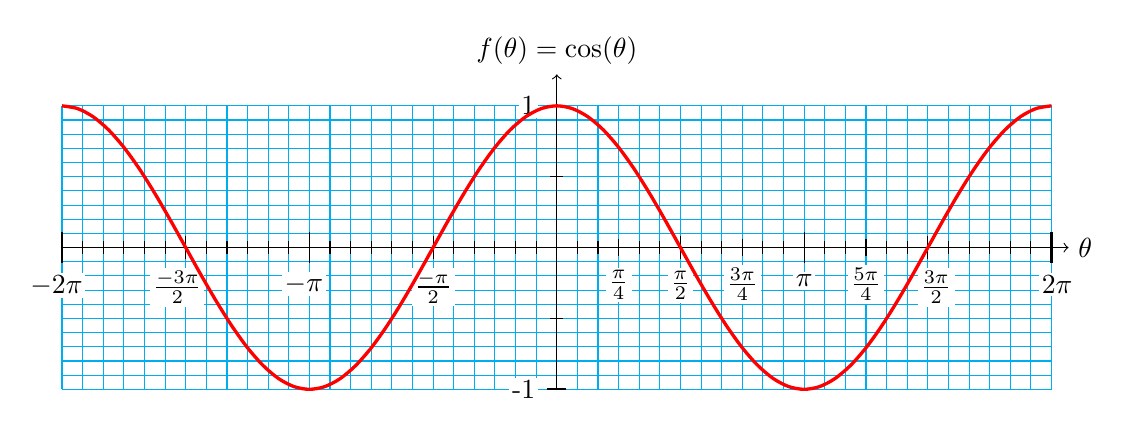
\begin{tikzpicture} 
\draw[cyan,xstep=pi/12,ystep=0.18]
(-2*pi,-1.8) grid (2*pi,1.8);

\draw[->] (-6.3,0) -- (6.5,0) node[right] {$\theta$};
\draw[->] (0,-1.8) -- (0,2.2) node[above] {$f(\theta)=\cos(\theta)$};

\foreach \x in {-24,-23,...,24}
\draw[black] ($ pi*\x /12*(1,0) +(0,.08) $) --++(0,-.16);
\foreach \y in {-0.9, 0.9}
\draw[black] (.08,\y ) --++(-.16,0);
\foreach \y in {-1,1}
\draw[black, thick] (.12,1.8*\y ) --++(-.24,0) node[anchor=east, xshift=-3, fill=white, inner sep=1pt] {\y};

\draw[black, thick] (-2*pi,.2) --++(0,-.4) node[anchor=north, xshift=-2,yshift=-3, fill=white, inner sep=1pt] {$-2\pi$};
\draw[black, thick] (2*pi,.2) --++(0,-.4) node[anchor=north, xshift=2,yshift=-3, fill=white, inner sep=1pt] {$2\pi$};

\draw[black] (pi,.2) --++(0,-.4) node[anchor=north, yshift=-3, fill=white, inner sep=1pt] {$\pi$};

\draw[black] (pi,.2) --++(0,-.4) node[anchor=north, yshift=-3, fill=white, inner sep=1pt] {$\pi$};
\draw[black] (-pi,.2) --++(0,-.4) node[anchor=north, xshift=-2,yshift=-3, fill=white, inner sep=1pt] {$-\pi$};
\draw[black] (-pi/2,.15) --++(0,-.3) node[anchor=north, yshift=-3, fill=white, inner sep=1pt] {$\frac{-\pi}{2}$};
\draw[black] (pi/2,.15) --++(0,-.3) node[anchor=north, yshift=-3, fill=white, inner sep=1pt] {$\frac{\pi}{2}$};
\draw[black] (3*pi/2,.15) --++(0,-.3) node[anchor=north,xshift=3, yshift=-3, fill=white, inner sep=1pt] {$\frac{3\pi}{2}$};
\draw[black] (-3*pi/2,.15) --++(0,-.3) node[anchor=north,xshift=-3, yshift=-3, fill=white, inner sep=1pt] {$\frac{-3\pi}{2}$};

\draw[black] (pi/4,.11) --++(0,-.22) node[anchor=north, yshift=-4, fill=white, inner sep=1pt] {$\frac{\pi}{4}$};

\draw[black] (3*pi/4,.11) --++(0,-.22) node[anchor=north, yshift=-3, fill=white, inner sep=1pt] {$\frac{3\pi}{4}$};

\draw[black] (5*pi/4,.11) --++(0,-.22) node[anchor=north, yshift=-3, fill=white, inner sep=1pt] {$\frac{5\pi}{4}$};

\draw[samples=65,domain=-2*pi:2*pi,smooth,variable=\x,red,very thick] plot ({\x},{1.8*cos(deg(\x))});

\end{tikzpicture}
\newline


fig-8-1-4 tangent graph
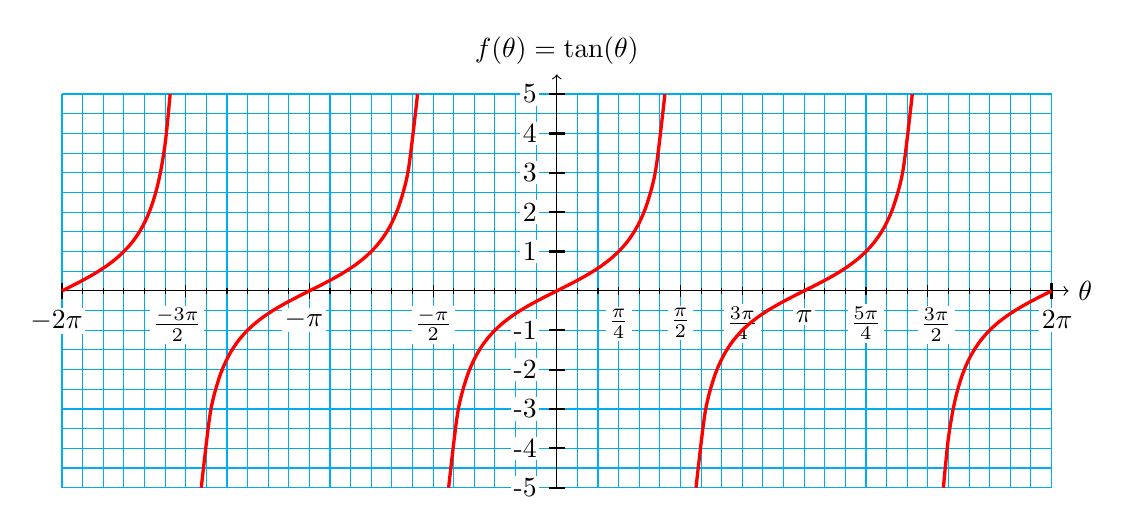
\begin{tikzpicture} [yscale=.5]
\draw[cyan,xstep=pi/12,ystep=0.5]
(-2*pi,-5) grid (2*pi,5);

\draw[->] (-6.3,0) -- (6.5,0) node[right] {$\theta$};
\draw[->] (0,-5) -- (0,5.5) node[above] {$f(\theta)=\tan(\theta)$};

\foreach \x in {-24,-23,...,24}
\draw[black] ($ pi*\x /12*(1,0) +(0,.08) $) --++(0,-.16);
\foreach \y in {-5,-4,...,-1,1,2,...,5}
\draw[black, thick] (.10,\y ) --++(-.2,0) node[anchor=east, xshift=-3, fill=white, inner sep=1pt] {\y};

\draw[black, thick] (-2*pi,.2) --++(0,-.4) node[anchor=north, xshift=-2,yshift=-3, fill=white, inner sep=1pt] {$-2\pi$};
\draw[black, thick] (2*pi,.2) --++(0,-.4) node[anchor=north, xshift=2,yshift=-3, fill=white, inner sep=1pt] {$2\pi$};

\draw[black] (pi,.2) --++(0,-.4) node[anchor=north, yshift=-3, fill=white, inner sep=1pt] {$\pi$};

\draw[black] (pi,.2) --++(0,-.4) node[anchor=north, yshift=-3, fill=white, inner sep=1pt] {$\pi$};
\draw[black] (-pi,.2) --++(0,-.4) node[anchor=north, xshift=-2,yshift=-3, fill=white, inner sep=1pt] {$-\pi$};
\draw[black] (-pi/2,.15) --++(0,-.3) node[anchor=north, yshift=-3, fill=white, inner sep=1pt] {$\frac{-\pi}{2}$};
\draw[black] (pi/2,.15) --++(0,-.3) node[anchor=north, yshift=-3, fill=white, inner sep=1pt] {$\frac{\pi}{2}$};
\draw[black] (3*pi/2,.15) --++(0,-.3) node[anchor=north,xshift=3, yshift=-3, fill=white, inner sep=1pt] {$\frac{3\pi}{2}$};
\draw[black] (-3*pi/2,.15) --++(0,-.3) node[anchor=north,xshift=-3, yshift=-3, fill=white, inner sep=1pt] {$\frac{-3\pi}{2}$};

\draw[black] (pi/4,.11) --++(0,-.22) node[anchor=north, yshift=-4, fill=white, inner sep=1pt] {$\frac{\pi}{4}$};

\draw[black] (3*pi/4,.11) --++(0,-.22) node[anchor=north, yshift=-3, fill=white, inner sep=1pt] {$\frac{3\pi}{4}$};

\draw[black] (5*pi/4,.11) --++(0,-.22) node[anchor=north, yshift=-3, fill=white, inner sep=1pt] {$\frac{5\pi}{4}$};

\foreach \i in {-1, 0, 1}
	\draw[domain={\i*pi-atan(5)*pi/180}:{\i*pi+atan(5)*pi/180}, smooth, variable=\x,red,very thick] plot ({\x},{tan(deg(\x))}) ;

\draw[domain={-2*pi:atan(5)*pi/180-2*pi}, smooth, variable=\x,red,very thick] plot ({\x},{tan(deg(\x))}) ;
\draw[domain={2*pi-atan(5)*pi/180:2*pi}, smooth, variable=\x,red,very thick] plot ({\x},{tan(deg(\x))}) ;

\end{tikzpicture}
\newline


exam8-1-6 right triangle
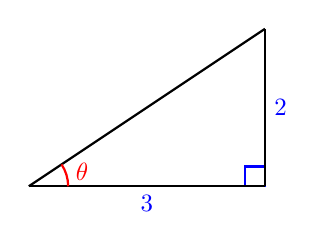
\begin{tikzpicture} 
\coordinate (O) at (0,0);
\coordinate (A) at (3,0);
\coordinate (B) at (3,2);
\draw[blue,thick] (A) rectangle ++(-.25, .25);
\draw[black,thick] (O)--(A) node[below, midway, scale=.9, text=blue] {3};
\draw[black,thick] (A)--(B) node[right, midway, scale=.9, text=blue] {2};
\draw[black,thick] (B)--(O);
\draw[red,thick] (0.5,0) arc(0:{atan(2/3)}:.5) node[right, yshift=1, midway, scale=.9] {$\theta$};
\end{tikzpicture}
\newline

exam8-1-7right triangle
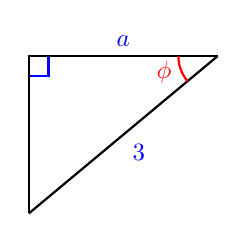
\begin{tikzpicture} 
\coordinate (O) at (0,0);
\coordinate (A) at (2.4,0);
\coordinate (B) at (0,-2);
\draw[blue,thick] (O) rectangle ++(.25, -.25);
\draw[black,thick] (O)--(A) node[above, midway, scale=.9, text=blue] {$a$};
\draw[black,thick] (A)--(B) node[below right, midway, scale=.9, text=blue] {3};
\draw[black,thick] (B)--(O);
\draw[red,thick] (1.9,0) arc(180:{180+atan(5/6)}:.5) node[left, yshift=-1, midway, scale=.9] {$\phi$};
\end{tikzpicture}
\newline


hp8-1-1ans angles 
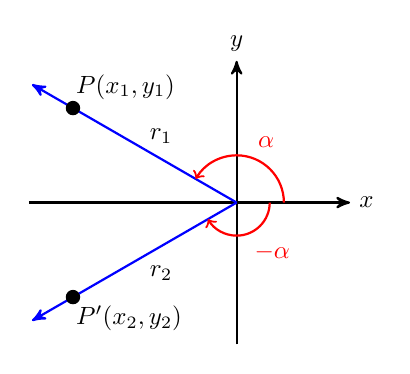
\begin{tikzpicture} [scale=1.2]
\draw[black,thick,->,>=stealth'] (-2.2,0)--(1.2,0) node[right,scale=.9] {$x$};
\draw[black,thick,->,>=stealth'] (0,-1.5)--(0,1.5) node[above,scale=.9] {$y$};
\coordinate (O) at (0,0);
\def\al{150};
\coordinate (P) at (\al:2);
\coordinate (Pp) at (-\al:2);
\coordinate (R) at (\al:2.5);
\coordinate (Rp) at (-\al:2.5);
\draw[blue,thick,->,>=stealth'] (O)--(R);
\draw[blue,thick,->,>=stealth'] (O)--(Rp);
\filldraw[black] (P) circle (2pt) node[above right, xshift=-2, scale=.9] {$P(x_1,y_1)$};
\filldraw[black] (Pp) circle (2pt) node[below right, xshift=-2, scale=.9] {$P'(x_2,y_2)$};
\draw[red,thick,->] (0.5,0) arc(0:{\al}:0.5) node[above right, midway, scale=.9] {$\alpha$};
\draw[red,thick,->] (0.35,0) arc(0:{-\al}:0.35) node[below right, midway, scale=.9] {$-\alpha$};
\node[scale=.9] at (-0.8,0.7) {$r_1$};
\node[scale=.9] at (-0.8,-0.75) {$r_2$};
\end{tikzpicture}
\newline


hp8-1-3ans angles 7pi/12 and -7pi/12
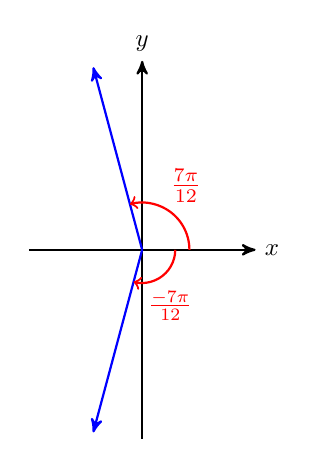
\begin{tikzpicture} [scale=1.2]
\draw[black,thick,->,>=stealth'] (-1.2,0)--(1.2,0) node[right,scale=.9] {$x$};
\draw[black,thick,->,>=stealth'] (0,-2)--(0,2) node[above,scale=.9] {$y$};
\coordinate (O) at (0,0);
\def\al{105};
\coordinate (R) at (\al:2.);
\coordinate (Rp) at (-\al:2.);
\draw[blue,thick,->,>=stealth'] (O)--(R);
\draw[blue,thick,->,>=stealth'] (O)--(Rp);
\draw[red,thick,->] (0.5,0) arc(0:{\al}:0.5) node[above right, xshift=-4, midway] {$\frac{7\pi}{12}$};
\draw[red,thick,->] (0.35,0) arc(0:{-\al}:0.35) node[below right, xshift=2, scale=.9] {$\frac{-7\pi}{12}$};
\end{tikzpicture}
\newline


hp8-1-11ans 

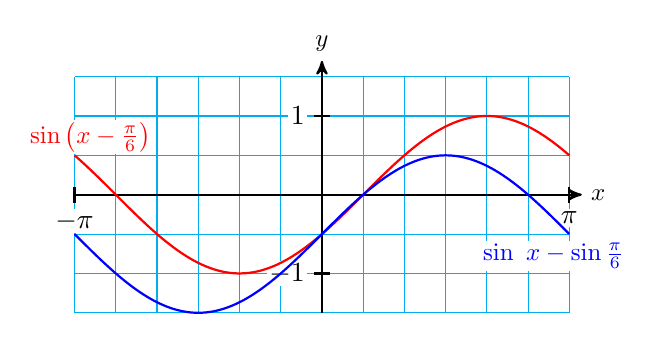
\begin{tikzpicture}
\draw[cyan] (-pi,-3/2) grid[xstep=pi/6,ystep=1/2] (pi,3/2);
\draw[black,thick,->,>=stealth'] (-pi,0)--(3.3,0) node[right,scale=.9] {$x$};
\draw[black,thick,->,>=stealth'] (0,-3/2)--(0,1.7) node[above,scale=.9] {$y$};
\draw[black,thick] (-pi,.1)--++(0,-.2) node[below, yshift=-2, fill=white, inner sep=1] {$-\pi$};
\draw[black,thick] (pi,.1)--++(0,-.2) node[below, yshift=-2, fill=white, inner sep=1] {$\pi$};
\foreach \y in {-1,1} \draw[black,thick] (.1,\y)--++(-.2,0) node[left, xshift=-2, fill=white, inner sep=1] {$\y$};
\draw[samples=65,domain=pi:-pi, variable=\x, smooth, thick, red] plot(\x, {sin( deg(\x-pi/6) )}) node[above, xshift=.2cm,fill=white, inner sep=1, scale=.9] {$\sin\left(x-\frac{\pi}{6}\right)$} ;
\draw[samples=65,domain=-pi:pi, variable=\x, smooth, thick, blue] plot(\x, {sin( deg(\x) )-1/2}) node[below, xshift=-.2cm, yshift=-2
,fill=white, inner sep=1, scale=.9] {$\sin\ x-\sin \frac{\pi}{6}$} ;
\end{tikzpicture}
\newline


hp8-1-19ans angles

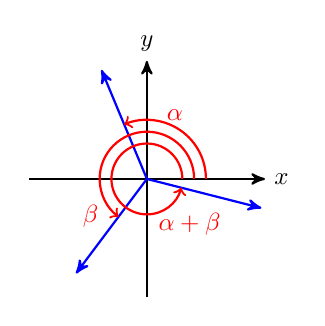
\begin{tikzpicture} [scale=1.5]
\coordinate (O) at (0,0);
\def\as{180-asin(12/13)};
\coordinate (A) at ({\as}:1);
\def\ac{360-acos(-3/5)};
\coordinate (B) at ({\ac}:1);
\def\sa{\as+\ac});
\coordinate(C) at ({\sa}:1);
\draw[black,thick,->,>=stealth'] (-1,0)--(1,0) node[right,scale=.9]{$x$};
\draw[black,thick,->,>=stealth'] (0,-1)--(0,1) node[above,scale=.9]{$y$};
\draw[blue,thick,->,>=stealth'] (O)--(A);
\draw[red,thick,->] (0.5, 0) arc(0:{\as}:0.5) node[above right, xshift=-8, midway, scale=.9] {$\alpha$};
\draw[blue,thick,->,>=stealth'] (O)--(B);
\draw[red,thick,->] (0.4, 0) arc(0:{\ac}:0.4) node[left, xshift=-4,  scale=.9] {$\beta$};
\draw[blue,thick,->,>=stealth'] (O)--(C);
\draw[red,thick,->] (0.3, 0) arc(0:{\sa}:0.3) node[below, xshift=3, yshift=-6,  scale=.9] {$\alpha+\beta$};

\end{tikzpicture}
\newline




fig-4-2-unitcircle
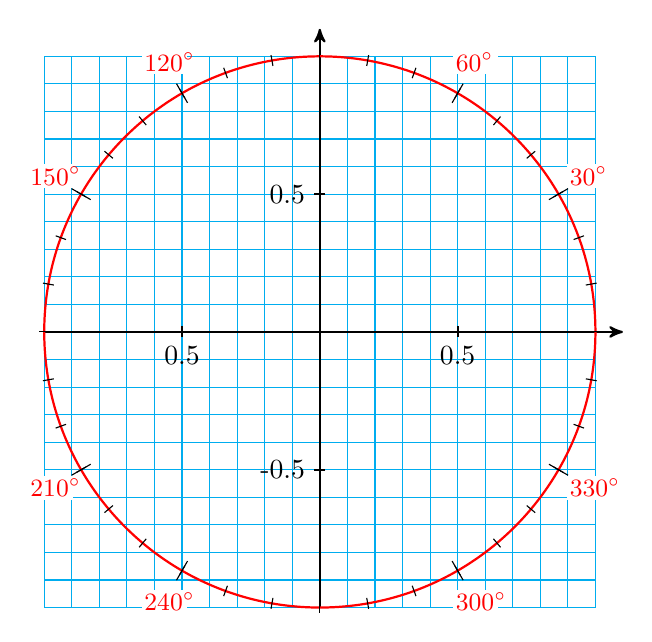
\begin{tikzpicture} [scale = .35] 
\draw[cyan] (-10,-10) grid (10,10);
\draw[black,thick,->,>=stealth'] (-10,0)--(11,0);
\draw[black,thick,->,>=stealth'] (0,-10)--(0,11);
\coordinate (O) at (0,0);
\draw[red,thick] (O) circle (10cm);
\foreach \theta  in {0,10,...,360}
\draw[black] (\theta: 9.8)--(\theta:10.2)  ;
\draw[black,  thick] (5,0.2) --++(0,-0.4) node[below, yshift=-2, inner sep=1] {0.5};
\draw[black,  thick] (-5,0.2) --++(0,-0.4) node[below, yshift=-2, inner sep=1] {0.5};
\draw[black,  thick] (0.2,5) --++(-0.4,0) node[left, xshift=-2, inner sep=1] {0.5};
\draw[black,  thick] (0.2,-5) --++(-0.4,0) node[left, xshift=-2, inner sep=1] {-0.5};
\foreach \theta  in {30, 60, 120, 150, 210, 240, 300, 330}
{
\draw[black] (\theta: 9.6)--(\theta:10.4) ;
\node[text width=0.5cm, color=red,fill=white, inner sep=1pt] at (\theta:11.3) {\small $\theta\degree$};
};
\end{tikzpicture}
\newline


hp8-1-55 two triangles

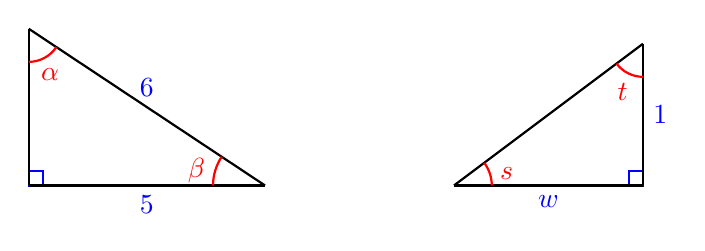
\begin{tikzpicture} [scale=.6]
\coordinate (C) at (0,0);
\coordinate (A) at (5,0);
\coordinate (B) at ($ sqrt(11)*(0,1) $);
\draw[blue,thick] (C) rectangle ++(.3,.3);
\draw[black,thick] (C)--(A) node[below, midway, text=blue] {5};
\draw[black,thick] (B)--(A) node[above, midway, text=blue] {6};
\draw[black,thick] (C)--(B);
\draw[red,thick] ($ sqrt(11)*(0,1) + (0,-0.7) $) arc(-90:{-acos(5/6)}:0.7) node[below, xshift=2, midway] {$\alpha$};
\draw[red,thick] (3.9,0) arc(180:{180-acos(5/6)}:1.1) node[left, midway] {$\beta$};

%second triangle
\def\sh{13};
\coordinate (F) at (\sh,0);
\coordinate (D) at ($ \sh*(1,0)+ (-4,0) $);
\coordinate (E) at ($ \sh*(1,0)+ (0,3) $);
\draw[blue,thick] (F) rectangle ++(-.3,.3);
\draw[black,thick] (F)--(D) node[below, midway, text=blue] {$w$};
\draw[black,thick] (E)--(D);
\draw[black,thick] (F)--(E) node[right, midway, text=blue] {1};
\draw[red,thick] ($ \sh*(1,0) + (0,2.3) $) arc(270:{180+atan(3/4)}:0.7) node[below, xshift=-2, midway] {$t$};
\draw[red,thick] ($ \sh*(1,0) +(-3.2,0) $) arc(0:{atan(3/4)}:0.8) node[right, midway] {$s$};
\end{tikzpicture}
\newline


hp8-1-59ans angles

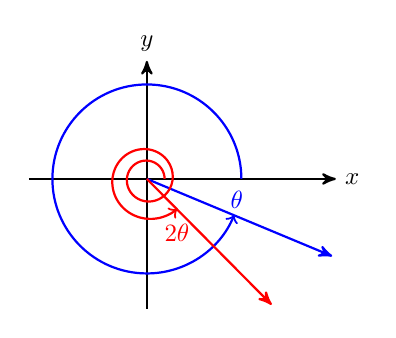
\begin{tikzpicture} [scale=1.5]
\coordinate (O) at (0,0);
\def\th{360-acos(12/13)};
\coordinate (A) at ({\th}:1.7);
\def\an{720-2*acos(12/13)};
\coordinate (B) at ({\an}:1.5);
\draw[black,thick,->,>=stealth'] (-1,0)--(1.6,0) node[right,scale=.9]{$x$};
\draw[black,thick,->,>=stealth'] (0,-1.1)--(0,1) node[above,scale=.9]{$y$};
\draw[blue,thick,->,>=stealth'] (O)--(A);
\draw[blue,thick,->] (0.8, 0) arc(0:{\th}:0.8) node[above, xshift=1, yshift=-1, scale=.9] {$\theta$};
\draw[red,thick,->,>=stealth'] (O)--(B);
\draw [domain=0:{4*pi - 2*acos(12/13)*pi/180 },variable=\t, smooth, samples=75,->, below, red, thick] plot ({\t r}: {.15+\t^(1.8) /400 }) node[below, yshift=-2, scale=.9] {$2\theta$};;

\end{tikzpicture}
\newline


hp8-1-89 triangle inscribed in rectangle

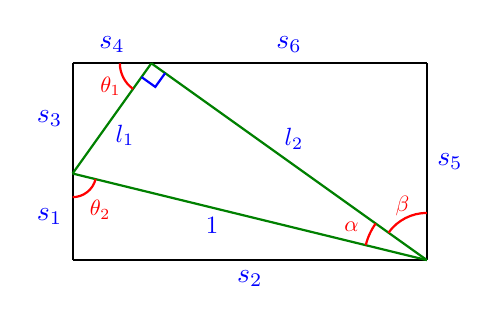
\begin{tikzpicture}
\coordinate (O) at (0,0);
\coordinate (A) at (4.5,0);
\coordinate (B) at (4.5,2.5);
\coordinate (C) at (0,2.5);
\coordinate (P) at (0,1.1);
\coordinate (Q) at (1,2.5);
\draw[black,thick] (O)--(A) node[below,midway, text=blue] {$s_2$};
\draw[black,thick] (B)--(A) node[right,midway, text=blue] {$s_5$};
\draw[black,thick] (B)--(Q) node[above,midway, text=blue] {$s_6$};
\draw[black,thick] (C)--(Q) node[above,midway, text=blue] {$s_4$};
\draw[black,thick] (C)--(P) node[left,midway, text=blue] {$s_3$};
\draw[black,thick] (O)--(P) node[left,midway, text=blue] {$s_1$};
\draw[green!50!black,thick] (A)--(P) node[below left, xshift=-8, yshift=3,midway, text=blue, scale=.9] {$1$};
\draw[green!50!black,thick] (A)--(Q) node[above right, xshift=-5, yshift=1,midway, text=blue, scale=.9] {$l_2$};
\draw[green!50!black,thick] (P)--(Q) node[below right, xshift=-2, yshift=1,midway, text=blue, scale=.9] {$l_1$};
\draw[blue,thick] (Q)++(.175,-.125)--++(-.125,-.175)--++(-.175,.125);

\draw[red,thick] (Q)++(-.4,0) arc(180:{180+atan(7/5)}:.4) node[left, xshift=2, yshift=-3, midway, scale=.8] {$\theta_1$};
\draw[red,thick] (P)++(0,-.3) arc(270:{270+atan(45/11)}:.3) node[below right, xshift=-2, midway, scale=.8] {$\theta_2$};
\draw[red,thick] (A)++({180-atan(11/45}:0.8) arc({180-atan(11/45)}:{90+atan(7/5)}:.8) node[above left, xshift=-1, yshift=-2, midway, scale=.8] {$\alpha$};
\draw[red,thick] (A)++(0,.6) arc(90:{90+atan(7/5)}:.6) node[above , xshift=-1, yshift=-2, midway, scale=.8] {$\beta$};

\end{tikzpicture}
\newline


hp8-1-89ans triangle inscribed in rectangle

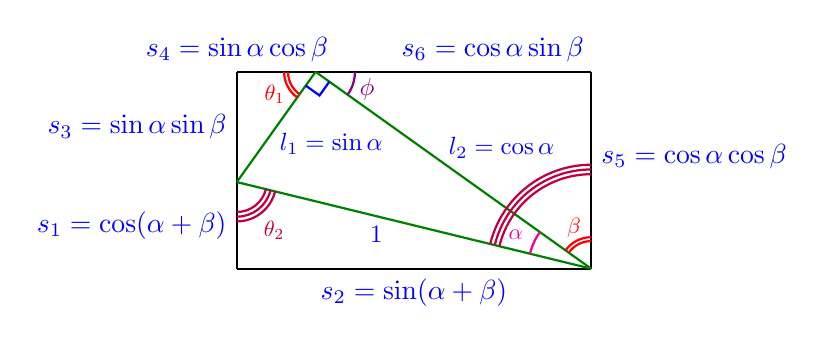
\begin{tikzpicture}
\coordinate (O) at (0,0);
\coordinate (A) at (4.5,0);
\coordinate (B) at (4.5,2.5);
\coordinate (C) at (0,2.5);
\coordinate (P) at (0,1.1);
\coordinate (Q) at (1,2.5);
\draw[black,thick] (O)--(A) node[below,midway, text=blue] {$s_2=\sin(\alpha+\beta) $};
\draw[black,thick] (B)--(A) node[right, yshift=5,midway, text=blue] {$s_5=\cos\alpha\cos\beta$};
\draw[black,thick] (B)--(Q) node[above,midway, xshift=.5cm, text=blue] {$s_6=\cos\alpha\sin\beta$};
\draw[black,thick] (C)--(Q) node[above,midway, xshift=-.5cm, text=blue] {$s_4=\sin\alpha\cos\beta$};
\draw[black,thick] (C)--(P) node[left,midway, text=blue] {$s_3=\sin\alpha\sin\beta$};
\draw[black,thick] (O)--(P) node[left,midway, text=blue] {$s_1=\cos(\alpha+\beta)$};
\draw[green!50!black,thick] (A)--(P) node[below left, xshift=-8, yshift=3,midway, text=blue, scale=.9] {$1$};
\draw[green!50!black,thick] (A)--(Q) node[above right, xshift=-5, yshift=1,midway, text=blue, scale=.9] {$l_2=\cos\alpha$};
\draw[green!50!black,thick] (P)--(Q) node[below right, xshift=-2, yshift=1,midway, text=blue, scale=.9] {$l_1=\sin\alpha$};
\draw[blue,thick] (Q)++(.175,-.125)--++(-.125,-.175)--++(-.175,.125);

\draw[red,thick] (Q)++(-.35,0) arc(180:{180+atan(7/5)}:.35);
\draw[red,thick] (Q)++(-.4,0) arc(180:{180+atan(7/5)}:.4) node[left, xshift=2, yshift=-3, midway, scale=.8] {$\theta_1$};
\draw[purple,thick] (P)++(0,-.38) arc(270:{270+atan(45/11)}:.38) ;
\draw[purple,thick] (P)++(0,-.44) arc(270:{270+atan(45/11)}:.44) ;
\draw[purple,thick] (P)++(0,-.5) arc(270:{270+atan(45/11)}:.5) node[below right, xshift=-2, midway, scale=.8] {$\theta_2$};
\draw[magenta,thick] (A)++({180-atan(11/45}:0.8) arc({180-atan(11/45)}:{90+atan(7/5)}:.8) node[above left, xshift=-1, yshift=-2, midway, scale=.8] {$\alpha$};
\draw[red,thick] (A)++(0,.35) arc(90:{90+atan(7/5)}:.35);
\draw[red,thick] (A)++(0,.4) arc(90:{90+atan(7/5)}:.4) node[above , xshift=-1, yshift=-2, midway, scale=.8] {$\beta$};
\draw[violet,thick] (Q)++(0.5,0) arc(0:{-atan(5/7)}:.5) node[right , xshift=-1, yshift=-2, midway, scale=.9] {$\phi$};
\draw[purple,thick]  (A)++(0,1.2) arc(90:{90+atan(45/11)}:1.2);
\draw[purple,thick]  (A)++(0,1.26) arc(90:{90+atan(45/11)}:1.26);
\draw[purple,thick]  (A)++(0,1.32) arc(90:{90+atan(45/11)}:1.32);

\end{tikzpicture}
\newline


hp8-1-90 triangle inscribed in rectangle

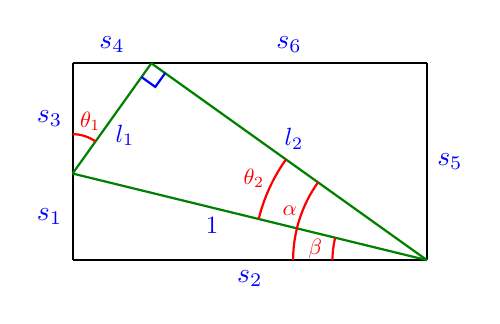
\begin{tikzpicture}
\coordinate (O) at (0,0);
\coordinate (A) at (4.5,0);
\coordinate (B) at (4.5,2.5);
\coordinate (C) at (0,2.5);
\coordinate (P) at (0,1.1);
\coordinate (Q) at (1,2.5);
\draw[black,thick] (O)--(A) node[below,midway, text=blue] {$s_2$};
\draw[black,thick] (B)--(A) node[right,midway, text=blue] {$s_5$};
\draw[black,thick] (B)--(Q) node[above,midway, text=blue] {$s_6$};
\draw[black,thick] (C)--(Q) node[above,midway, text=blue] {$s_4$};
\draw[black,thick] (C)--(P) node[left,midway, text=blue] {$s_3$};
\draw[black,thick] (O)--(P) node[left,midway, text=blue] {$s_1$};
\draw[green!50!black,thick] (A)--(P) node[below left, xshift=-8, yshift=3,midway, text=blue, scale=.9] {$1$};
\draw[green!50!black,thick] (A)--(Q) node[above right, xshift=-5, yshift=1,midway, text=blue, scale=.9] {$l_2$};
\draw[green!50!black,thick] (P)--(Q) node[below right, xshift=-2, yshift=1,midway, text=blue, scale=.9] {$l_1$};
\draw[blue,thick] (Q)++(.175,-.125)--++(-.125,-.175)--++(-.175,.125);

\draw[red,thick] (P)++(0,.5) arc(90:{90-atan(5/7)}:.5) node[above, xshift=2, yshift=-1, midway, scale=.8] {$\theta_1$};
\draw[red,thick] (A)++({180-atan(11/45}:2.2) arc({180-atan(11/45)}:{90+atan(7/5)}:2.2) node[above left, xshift=1, yshift=-3, midway, scale=.8] {$\theta_2$};
\draw[red,thick] (A)++(-1.7,0) arc({180}:{90+atan(7/5)}:1.7) node[left, xshift=2, yshift=3, midway, scale=.8] {$\alpha$};
\draw[red,thick] (A)++(-1.2,0) arc(180:{180-atan(11/45)}:1.2) node[left,, midway, xshift=-1, yshift=0, midway, scale=.8] {$\beta$};

\end{tikzpicture}
\newline


hp8-1-91 unit circle for cosine identity

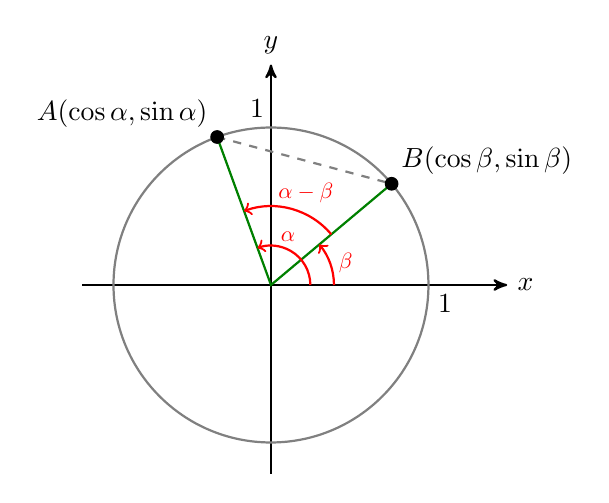
\begin{tikzpicture} [scale=2];
\coordinate (O) at (0,0);
\coordinate (B) at (40:1);
\coordinate (A) at (110:1);
\node[below right] at (1,0) {1};
\node[above left, xshift=1] at (0,1) {1};
\draw[black,thick,->,>=stealth'] (-1.2,0)--(1.5,0) node[right] {$x$};
\draw[black,thick,->,>=stealth'] (0,-1.2)--(0,1.4) node[above]{$y$};
\draw[gray,thick] (O) circle (1cm);
\draw[green!50!black, thick] (A)--(O)--(B);
\draw[gray,thick,dashed] (A)--(B);
\filldraw[black] (A) circle (.04cm) node[above left]{$A(\cos\alpha , \sin\alpha )$};
\filldraw[black] (B) circle (.04cm) node[above right]{$B(\cos\beta , \sin\beta )$};

\draw[red,thick,->] (0.25,0) arc(0:110:0.25) node[above, midway, xshift=-2, yshift=3,fill=white, inner sep=1, scale=0.8] {$\alpha$};
\draw[red,thick,->] (0.4,0) arc(0:40:0.4) node[right, xshift=2, midway,fill=white, inner sep=1, scale=0.8] {$\beta$};
\draw[red,thick,->] (40:0.5) arc(40:110:0.5) node[above right, xshift=-5, yshift=2, midway,fill=white, inner sep=0, scale=0.8] {$\alpha-\beta$};
\end{tikzpicture};
\newline


fig-8-2-2 $x^3$ and $\sqrt[3]{x}$

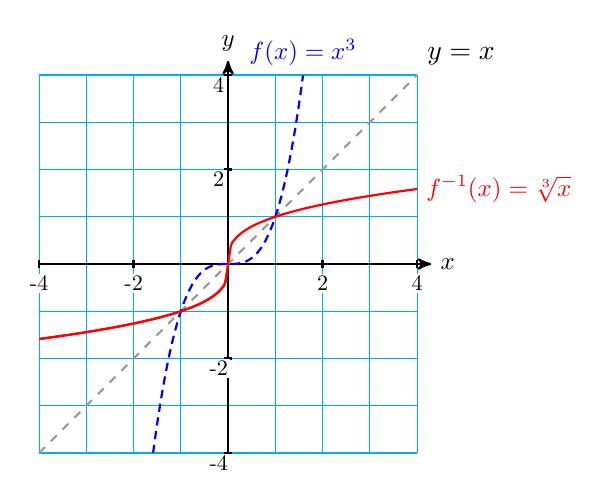
\begin{tikzpicture} [scale=.6]
\draw[cyan] (-4,-4) grid (4,4);
\draw[black,thick,->,>=stealth'] (-4,0)--(4.3,0) node[right, scale=.9] {$x$};
\draw[black,thick,->,>=stealth'] (0,-4)--(0,4.3) node[above, scale=.9] {$y$};
\foreach \x in {-4, -2, 2, 4} {
  \draw[black,thick] (\x, .08)--++(0,-.16) node[below, yshift=-2, fill=white, inner sep=1, scale=.8] {\x};
  \draw[black,thick] ( .08,\x)--++(-.16,0) node[below, xshift=-2, fill=white, inner sep=1, scale=.8] {\x};
};
\draw[gray!80!, thick, dashed] (-4,-4)--(4,4) node[above right, text=black] {$y=x$};
\draw[samples=65, domain=0:4, variable=\x, smooth, red, thick] plot (-\x, {-(\x)^(1/3)});
\draw[samples=65, domain={-4^(1/3)}:{4^(1/3)}, variable=\x, smooth, blue,thick,densely dashed] plot (\x, {(\x)^3}) node[above, scale=.9] {$f(x)=x^3$};
\draw[samples=65, domain=0:4, variable=\x, smooth, red, thick] plot (-\x, {-(\x)^(1/3)});
\draw[samples=65, domain=0:4, variable=\x, smooth, red, thick] plot (\x, {(\x)^(1/3)}) node[right, scale=.9] {$f^{-1}(x)=\sqrt[3]{x}$};
\end{tikzpicture}
\newline


exam8-2-2 translations of reciprocal function

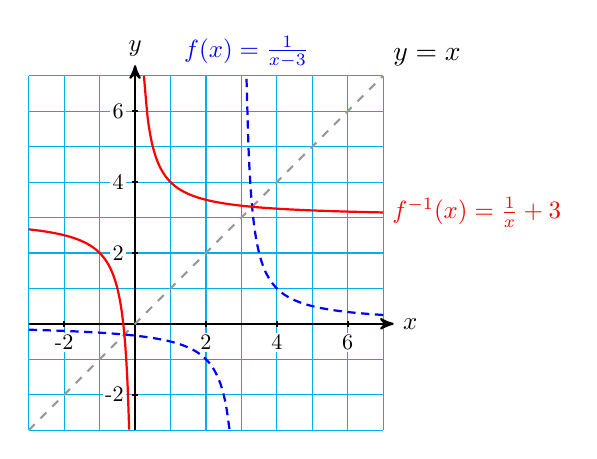
\begin{tikzpicture} [scale=.45]
\draw[cyan] (-3,-3) grid (7,7);
\draw[black,thick,->,>=stealth'] (-3,0)--(7.3,0) node[right, scale=.9] {$x$};
\draw[black,thick,->,>=stealth'] (0,-3)--(0,7.3) node[above, scale=.9] {$y$};
\foreach \x in { -2, 2, 4,6} {
  \draw[black,thick] (\x, .08)--++(0,-.16) node[below, yshift=-2, fill=white, inner sep=1, scale=.8] {\x};
  \draw[black,thick] ( .08,\x)--++(-.16,0) node[left, xshift=-2, fill=white, inner sep=1, scale=.8] {\x};
};
\draw[gray!80!, thick, dashed] (-3,-3)--(7,7) node[above right, text=black] {$y=x$};
\draw[samples=65, domain=-3:{3-1/3}, variable=\x, smooth, blue, thick, densely dashed] plot (\x, {1/(\x-3)});
\draw[samples=65, domain=7:{3+1/7)}, variable=\x, smooth, blue,thick,densely dashed] plot (\x, {1/(\x-3)}) node[above, scale=.9] {$f(x)=\frac{1}{x-3}$};
\draw[samples=65, domain=-3:-1/6, variable=\x, smooth, red, thick] plot (\x, {1/(\x) +3 });
\draw[samples=65, domain=1/4:7, variable=\x, smooth, red, thick] plot (\x, {1/(\x) +3}) node[right, scale=.9] {$f^{-1}(x)=\frac{1}{x}+3$};
\end{tikzpicture}
\newline


exam8-2-2alternate translations of reciprocal function

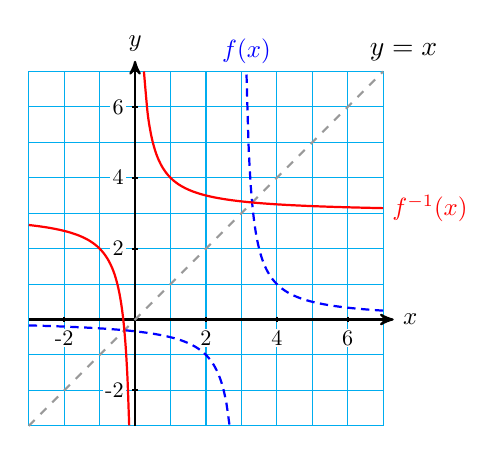
\begin{tikzpicture} [scale=.45]
\draw[cyan] (-3,-3) grid (7,7);
\draw[black,thick,->,>=stealth'] (-3,0)--(7.3,0) node[right, scale=.9] {$x$};
\draw[black,thick,->,>=stealth'] (0,-3)--(0,7.3) node[above, scale=.9] {$y$};
\foreach \x in { -2, 2, 4,6} {
  \draw[black,thick] (\x, .08)--++(0,-.16) node[below, yshift=-2, fill=white, inner sep=1, scale=.8] {\x};
  \draw[black,thick] ( .08,\x)--++(-.16,0) node[left, xshift=-2, fill=white, inner sep=1, scale=.8] {\x};
};
\draw[gray!80!, thick, dashed] (-3,-3)--(7,7) node[above right, xshift=-.3cm, text=black] {$y=x$};
\draw[samples=65, domain=-3:{3-1/3}, variable=\x, smooth, blue, thick, densely dashed] plot (\x, {1/(\x-3)});
\draw[samples=65, domain=7:{3+1/7)}, variable=\x, smooth, blue,thick,densely dashed] plot (\x, {1/(\x-3)}) node[above, scale=.9] {$f(x)$};
\draw[samples=65, domain=-3:-1/6, variable=\x, smooth, red, thick] plot (\x, {1/(\x) +3 });
\draw[samples=65, domain=1/4:7, variable=\x, smooth, red, thick] plot (\x, {1/(\x) +3}) node[right, scale=.9] {$f^{-1}(x)$};
\end{tikzpicture}
\newline


fig-8grid 8x8 grid
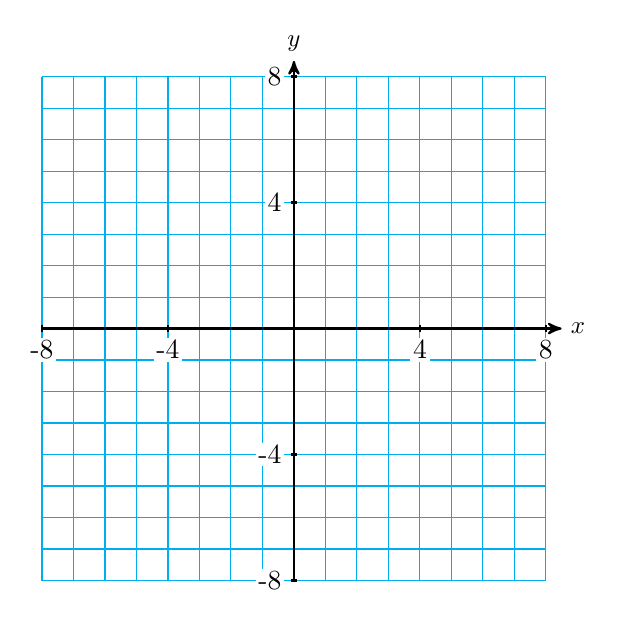
\begin{tikzpicture} [scale=0.4]
\draw[cyan] (-8,-8) grid (8,8);
\draw[black,thick,->,>=stealth'] (-8,0)--(8.5,0) node[right, scale=.9] {$x$};
\draw[black,thick,->,>=stealth'] (0,-8)--(0,8.5) node[above, scale=.9] {$y$};
\foreach \x in {-8,-4,4,8} {
  \draw[black,thick] (\x,0.1)--++(0,-.2) node[below, yshift=-2, fill=white, inner sep=1] {\x};
  \draw[black,thick] (0.1,\x)--++(-.2,0) node[left, xshift=-2, fill=white, inner sep=1] {\x};
};
\end{tikzpicture}
\newline


fig-8-2-2ans linear function and inverse
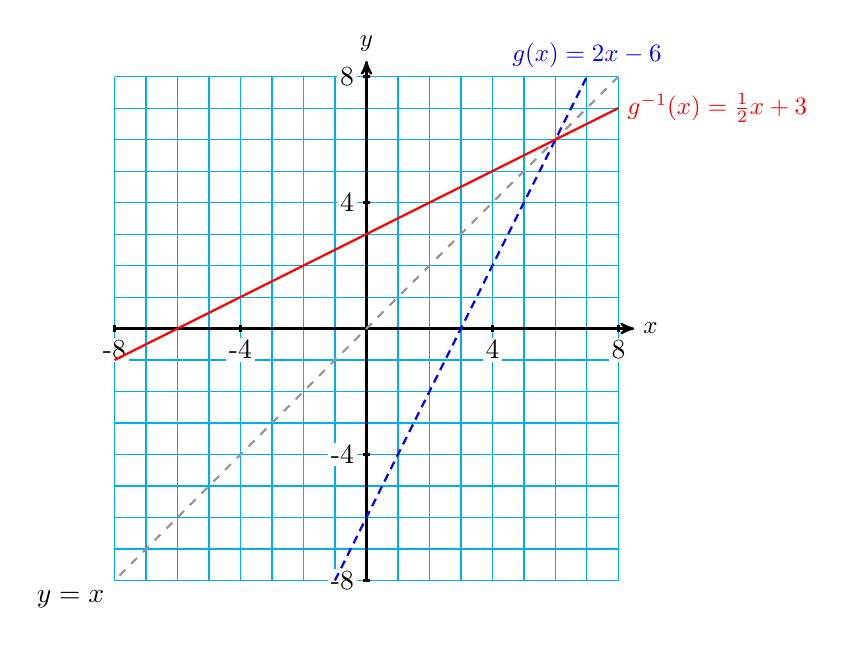
\begin{tikzpicture} [scale=0.4]
\draw[cyan] (-8,-8) grid (8,8);
\draw[black,thick,->,>=stealth'] (-8,0)--(8.5,0) node[right, scale=.9] {$x$};
\draw[black,thick,->,>=stealth'] (0,-8)--(0,8.5) node[above, scale=.9] {$y$};
\foreach \x in {-8,-4,4,8} {
  \draw[black,thick] (\x,0.1)--++(0,-.2) node[below, yshift=-2, fill=white, inner sep=1] {\x};
  \draw[black,thick] (0.1,\x)--++(-.2,0) node[left, xshift=-2, fill=white, inner sep=1] {\x};
};
\draw[gray!80!, thick, dashed] (8,8)--(-8,-8) node[below left, text=black] {$y=x$};
\draw[blue, densely dashed,thick] (-1,-8)--(7,8) node[above, scale=.9] {$g(x)=2x-6$};
\draw[red, thick] (-8,-1)--(8,7) node[right, scale=.9] {$g^{-1}(x)=\frac{1}{2}x+3 $};
\end{tikzpicture}
\newline

fig-8-2-3 parabolas

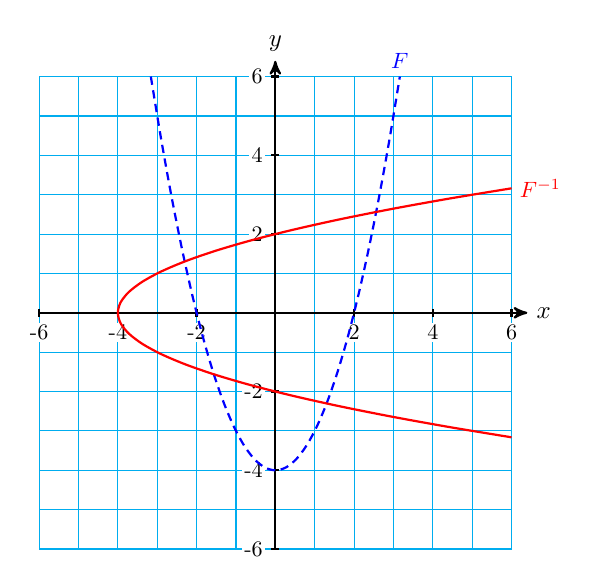
\begin{tikzpicture} [scale=1/2]
\draw[cyan] (-6,-6) grid (6,6);
\draw[black,thick,->,>=stealth'] (-6,0)--(6.4,0) node[right, scale=.9] {$x$};
\draw[black,thick,->,>=stealth'] (0,-6)--(0,6.4) node[above, scale=.9] {$y$};
\foreach \x in {-6,-4,-2,2,4,6} {
  \draw[black,thick] (\x,.1)--++(0,-.2) node[below, yshift=-2, fill=white, inner sep=1, scale=.8] {\x};
  \draw[black,thick] (.1,\x)--++(-.2,0) node[left, xshift=-2, fill=white, inner sep=1, scale=.8] {\x};
};
\draw[domain={-sqrt(10)}:{sqrt(10)},smooth, blue, thick, densely dashed] plot (\x, {(\x)^2-4}) node[above, scale=.8] {$F$};
\draw[domain={-sqrt(10)}:{sqrt(10)},smooth, red, thick] plot ( {(\x)^2-4}, \x) node[right, scale=.8] {$F^{-1}$};
\end{tikzpicture}
\newline


exam8-2-3 three graphs

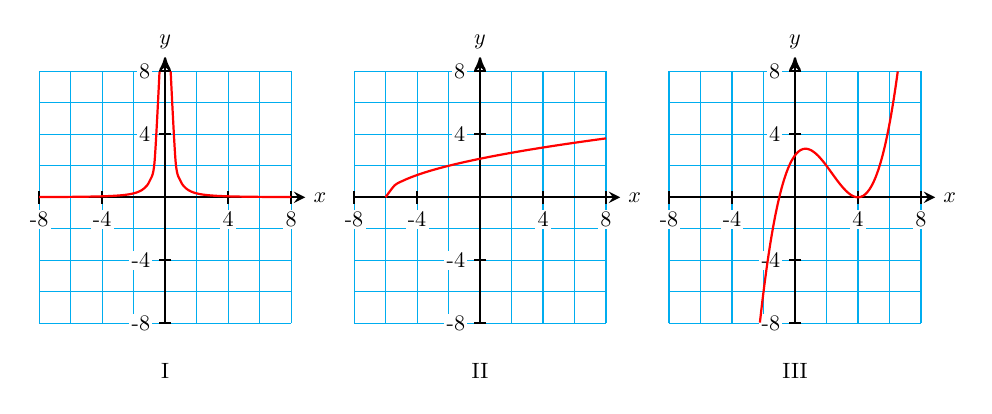
\begin{tikzpicture} [scale=.2]
\draw[cyan] (-8,-8) grid[step=2] (8,8);
\draw[black,thick,->,>=stealth] (-8,0)--++(16.9,0) node[right, scale=.8] {$x$};
\draw[black,thick,->,>=stealth'] (0,-8)--++(0,16.9) node[above, scale=.8] {$y$};;
\foreach \x in {-8,-4,4,8}{
  \draw[black,thick] (\x,.4)--++(0,-.8) node[below, yshift=-2, fill=white, inner sep=1, scale=.8] {\x};
  \draw[black,thick] (.4,\x)--++(-.8,0) node[left, xshift=-2, fill=white, inner sep=1, scale=.8] {\x};
};
\node[scale=.8] at (0,-11) {I};
\draw[domain=-8:{-1/sqrt(8)}, variable=\x, smooth, red, thick] plot (\x,{1/(\x)^2});
\draw[domain={1/sqrt(8)}:8, variable=\x, smooth, red, thick] plot (\x,{1/(\x)^2});

%second grid
\def\del{20};
\draw[cyan] ($ (\del,0)+(-8,-8)$) grid[step=2] ($ (\del,0)+(8,8)$);
\draw[black,thick,->,>=stealth] ($ (\del,0)+(-8,0)$)--++(16.9,0) node[right, scale=.8] {$x$};
\draw[black,thick,->,>=stealth'] ($ (\del,0)+(0,-8)$)--++(0,16.9) node[above, scale=.8] {$y$};;
\foreach \x in {-8,-4,4,8}{
  \draw[black,thick] ($ (\del,0)+(\x,.4)$)--++(0,-.8) node[below, yshift=-2, fill=white, inner sep=1, scale=.8] {\x};
  \draw[black,thick] ($ (\del,0)+(.4,\x)$)--++(-.8,0) node[left, xshift=-2, fill=white, inner sep=1, scale=.8] {\x};
};
\node[scale=.8] at ($ (\del,0)+(0,-11)$) {II};
\draw[,domain={-6}:{8}, variable=\x, smooth, red, thick] plot ({\x+\del},{sqrt(\x+6)});

%third grid
\def\del{40};
\draw[cyan] ($ (\del,0)+(-8,-8)$) grid[step=2] ($ (\del,0)+(8,8)$);
\draw[black,thick,->,>=stealth] ($ (\del,0)+(-8,0)$)--++(16.9,0) node[right, scale=.8] {$x$};
\draw[black,thick,->,>=stealth'] ($ (\del,0)+(0,-8)$)--++(0,16.9) node[above, scale=.8] {$y$};;
\foreach \x in {-8,-4,4,8}{
  \draw[black,thick] ($ (\del,0)+(\x,.4)$)--++(0,-.8) node[below, yshift=-2, fill=white, inner sep=1, scale=.8] {\x};
  \draw[black,thick] ($ (\del,0)+(.4,\x)$)--++(-.8,0) node[left, xshift=-2, fill=white, inner sep=1, scale=.8] {\x};
};
\node[scale=.8] at ($ (\del,0)+(0,-11)$) {III};
\draw[samples=65,domain={-2.23}:{6.525}, variable=\x, smooth, red, thick] plot ({\x+\del},{(\x+1)*(\x-4)^2 /6});

\end{tikzpicture}
\newline


exer8-2-3 three graphs

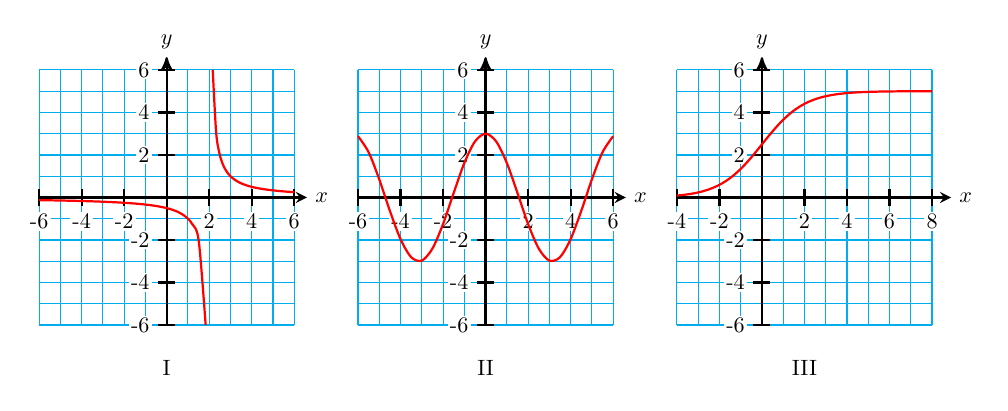
\begin{tikzpicture} [scale=.27]
\draw[cyan] (-6,-6) grid[step=1] (6,6);
\draw[black,thick,->,>=stealth] (-6,0)--++(12.6,0) node[right, scale=.8] {$x$};
\draw[black,thick,->,>=stealth'] (0,-6)--++(0,12.6) node[above, scale=.8] {$y$};;
\foreach \x in {-6,-4,-2,2,4,6}{
  \draw[black,thick] (\x,.4)--++(0,-.8) node[below, yshift=-2, fill=white, inner sep=1, scale=.8] {\x};
  \draw[black,thick] (.4,\x)--++(-.8,0) node[left, xshift=-2, fill=white, inner sep=1, scale=.8] {\x};
};
\node[scale=.8] at (0,-8) {I};
\draw[domain=-6:{2-1/6}, variable=\x, smooth, red, thick] plot (\x,{1/(\x-2)});
\draw[domain={13/6}:6, variable=\x, smooth, red, thick] plot (\x,{1/(\x-2)});

%second grid
\def\del{15};
\draw[cyan] ($ (\del,0)+(-6,-6)$) grid[step=1] ($ (\del,0)+(6,6)$);
\draw[black,thick,->,>=stealth] ($ (\del,0)+(-6,0)$)--++(12.6,0) node[right, scale=.8] {$x$};
\draw[black,thick,->,>=stealth'] ($ (\del,0)+(0,-6)$)--++(0,12.6) node[above, scale=.8] {$y$};;
\foreach \x in {-6,-4,-2,2,4,6}{
  \draw[black,thick] ($ (\del,0)+(\x,.4)$)--++(0,-.8) node[below, yshift=-2, fill=white, inner sep=1, scale=.8] {\x};
  \draw[black,thick] ($ (\del,0)+(.4,\x)$)--++(-.8,0) node[left, xshift=-2, fill=white, inner sep=1, scale=.8] {\x};
};
\node[scale=.8] at ($ (\del,0)+(0,-8)$) {II};
\draw[,domain={-6}:{6}, variable=\x, smooth, red, thick] plot ({\x+\del},{3*cos(deg(\x))});

%third grid
\def\del{28};
\draw[cyan] ($ (\del,0)+(-4,-6)$) grid[step=1] ($ (\del,0)+(8,6)$);
\draw[black,thick,->,>=stealth] ($ (\del,0)+(-4,0)$)--++(12.9,0) node[right, scale=.8] {$x$};
\draw[black,thick,->,>=stealth'] ($ (\del,0)+(0,-6)$)--++(0,12.6) node[above, scale=.8] {$y$};;
\foreach \x in {-6,-4,-2,2,4,6}{
  \draw[black,thick] ($ (\del,0)+(.4,\x)$)--++(-.8,0) node[left, xshift=-2, fill=white, inner sep=1, scale=.8] {\x};
};
\foreach \x in {-4,-2,2,4,6,8}{
  \draw[black,thick] ($ (\del,0)+(\x,.4)$)--++(0,-.8) node[below, yshift=-2, fill=white, inner sep=1, scale=.8] {\x};
};
\node[scale=.8] at ($ (\del,0)+(2,-8)$) {III};
\draw[samples=65,domain={-4}:{8}, variable=\x, smooth, red, thick] plot ({\x+\del},{ 5*e^\x)/(1+e^(\x)  ) });

\end{tikzpicture}
\newline

fig-8-2-4 parabolas

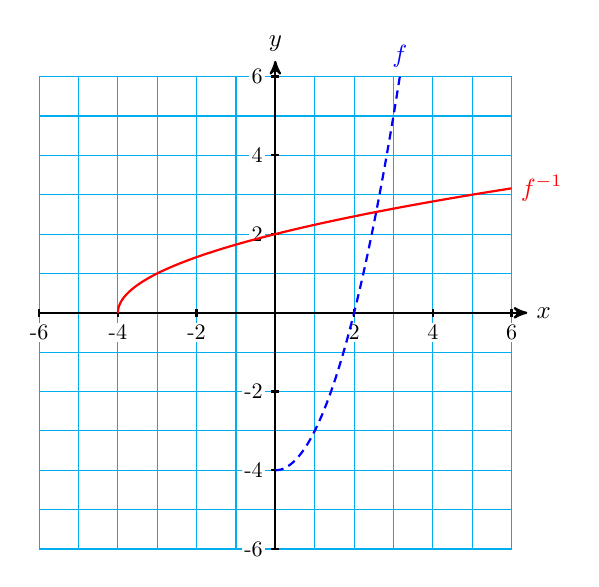
\begin{tikzpicture} [scale=1/2]
\draw[cyan] (-6,-6) grid (6,6);
\draw[black,thick,->,>=stealth'] (-6,0)--(6.4,0) node[right, scale=.9] {$x$};
\draw[black,thick,->,>=stealth'] (0,-6)--(0,6.4) node[above, scale=.9] {$y$};
\foreach \x in {-6,-4,-2,2,4,6} {
  \draw[black,thick] (\x,.1)--++(0,-.2) node[below, yshift=-2, fill=white, inner sep=1, scale=.8] {\x};
  \draw[black,thick] (.1,\x)--++(-.2,0) node[left, xshift=-2, fill=white, inner sep=1, scale=.8] {\x};
};
\draw[domain=0:{sqrt(10)},smooth, blue, thick, densely dashed] plot (\x, {(\x)^2-4}) node[above, scale=.9] {$f$};
\draw[domain=0:{sqrt(10)},smooth, red, thick] plot ( {(\x)^2-4}, \x) node[right, scale=.9] {$f^{-1}$};
\end{tikzpicture}
\newline

fig-8-2-5 restricted sine

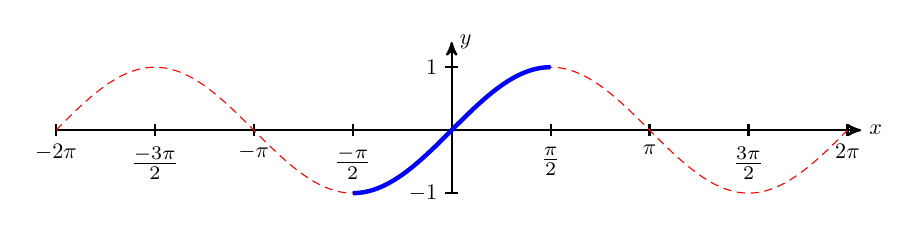
\begin{tikzpicture} [scale=.8]
\draw[black,thick,->,>=stealth'] (-2*pi,0)--(6.5,0) node[right, scale=.8] {$x$};
\draw[black,thick,->,>=stealth'] (0,-1)--(0,1.4) node[right, scale=.8] {$y$};
\foreach \y in {-1,1} \draw[black,thick] (.1,\y)--++(-.2,0) node[left, scale=.8] {$\y$};
\draw[black,thick] (-2*pi,0.1)--++(0,-.2) node [below, scale=.8] {$-2\pi$};
\draw[black,thick] (-3*pi/2,0.1)--++(0,-.2) node [below] {$\frac{-3\pi}{2} $};
\draw[black,thick] (-pi/2,0.1)--++(0,-.2) node [below] {$\frac{-\pi}{2} $};
\draw[black,thick] (-pi,0.1)--++(0,-.2) node [below, scale=.8] {$-\pi$};
\draw[black,thick] (pi/2,0.1)--++(0,-.2) node [below] {$\frac{\pi}{2} $};
\draw[black,thick] (pi,0.1)--++(0,-.2) node [below, scale=.8] {$\pi$};
\draw[black,thick] (3*pi/2,0.1)--++(0,-.2) node [below] {$\frac{3\pi}{2} $};
\draw[black,thick] (2*pi,0.1)--++(0,-.2) node [below, scale=.8] {$2\pi$};
\draw[samples=65,domain=-2*pi:2*pi,variable=\x, smooth, red, densely dashed] plot (\x,{sin(deg(\x))});
\draw[samples=65,domain=-pi/2:pi/2,variable=\x, smooth, blue, ultra thick] plot (\x,{sin(deg(\x))});
\end{tikzpicture}
\newline

fig-8-2-6 inverse sine

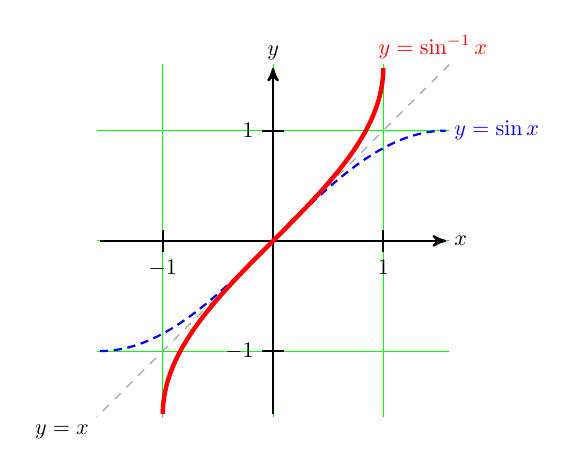
\begin{tikzpicture} [scale=1.4]
\draw[green] (-1.6,-1.6) grid (1.6,1.6);
\draw[black,thick,->,>=stealth'] (-pi/2,0)--(pi/2,0) node[right, scale=.8] {$x$};
\draw[black,thick,->,>=stealth'] (0,-pi/2)--(0,pi/2) node[above, scale=.8] {$y$};
\foreach \y in {-1,1} {
\draw[black,thick] (\y,.1)--++(0,-.2) node[below, scale=.8] {$\y$};
\draw[black,thick] (.1,\y)--++(-.2,0) node[left, scale=.8] {$\y$};
};
\draw[gray!80!white, dashed] (1.6,1.6)--(-1.6,-1.6) node[below left, scale=.8, text=black] {$y=x$};
\draw[samples=65,domain=-pi/2:pi/2,variable=\x, smooth, blue, thick, densely dashed] plot (\x,{sin(deg(\x))}) node[right, scale=.8] {$y=\sin x$};
\draw[samples=65,domain=-pi/2:pi/2,variable=\x, smooth, red, ultra thick] plot ({sin(deg(\x))},\x) node[above right, xshift=-5, scale=.8] {$y=\sin^{-1} x$};
\end{tikzpicture}
\newline

fig-8-2-7 restricted cosine

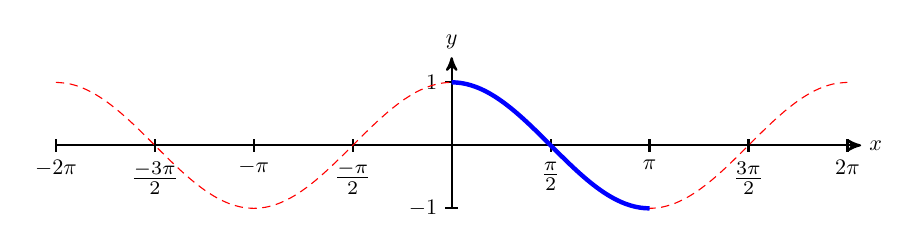
\begin{tikzpicture} [scale=.8]
\draw[black,thick,->,>=stealth'] (-2*pi,0)--(6.5,0) node[right, scale=.8] {$x$};
\draw[black,thick,->,>=stealth'] (0,-1)--(0,1.4) node[above, scale=.8] {$y$};
\foreach \y in {-1,1} \draw[black,thick] (.1,\y)--++(-.2,0) node[left, scale=.8] {$\y$};
\draw[black,thick] (-2*pi,0.1)--++(0,-.2) node [below, scale=.8] {$-2\pi$};
\draw[black,thick] (-3*pi/2,0.1)--++(0,-.2) node [below] {$\frac{-3\pi}{2} $};
\draw[black,thick] (-pi/2,0.1)--++(0,-.2) node [below] {$\frac{-\pi}{2} $};
\draw[black,thick] (-pi,0.1)--++(0,-.2) node [below, scale=.8] {$-\pi$};
\draw[black,thick] (pi/2,0.1)--++(0,-.2) node [below] {$\frac{\pi}{2} $};
\draw[black,thick] (pi,0.1)--++(0,-.2) node [below, scale=.8] {$\pi$};
\draw[black,thick] (3*pi/2,0.1)--++(0,-.2) node [below] {$\frac{3\pi}{2} $};
\draw[black,thick] (2*pi,0.1)--++(0,-.2) node [below, scale=.8] {$2\pi$};
\draw[samples=65,domain=-2*pi:2*pi,variable=\x, smooth, red, densely dashed] plot (\x,{cos(deg(\x))});
\draw[samples=65,domain=0:pi,variable=\x, smooth, blue, ultra thick] plot (\x,{cos(deg(\x))});
\end{tikzpicture}
\newline

fig-8-2-8 inverse sine

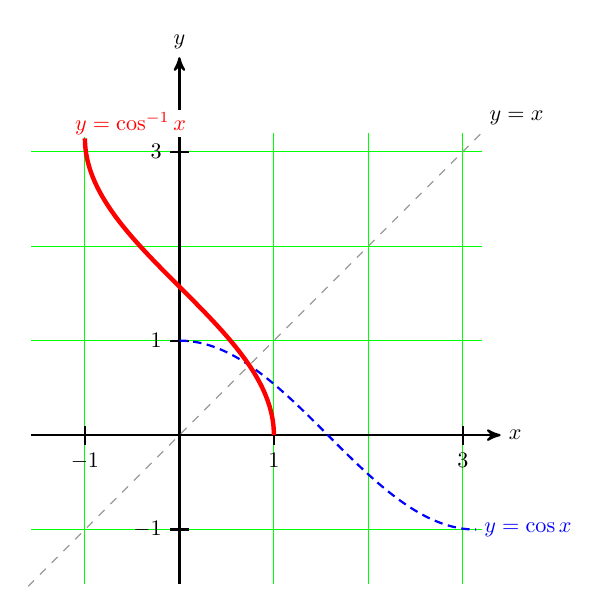
\begin{tikzpicture} [scale=1.2]
\draw[green] (-pi/2,-pi/2) grid (3.2,3.2);
\draw[black,thick,->,>=stealth'] (-pi/2,0)--(3.4,0) node[right, scale=.8] {$x$};
\draw[black,thick,->,>=stealth'] (0,-pi/2)--(0,4.) node[above, scale=.8] {$y$};
\foreach \y in {-1,1,3} {
\draw[black,thick] (\y,.1)--++(0,-.2) node[below, scale=.8] {$\y$};
\draw[black,thick] (.1,\y)--++(-.2,0) node[left, scale=.8] {$\y$};
};
\draw[gray!80!white, dashed] (-1.6,-1.6)--(3.2,3.2) node[above right, scale=.8, text=black] {$y=x$};
\draw[samples=65,domain=0:pi,variable=\x, smooth, blue, thick, densely dashed] plot (\x,{cos(deg(\x))}) node[right, scale=.8] {$y=\cos x$};
\draw[samples=65,domain=0:pi,variable=\x, smooth, red, ultra thick] plot ({cos(deg(\x))},\x) node[above right, xshift=-5, fill=white, inner sep=1, scale=.8] {$y=\cos^{-1} x$};
\end{tikzpicture}
\newline

fig-8-2-9 restricted tangent

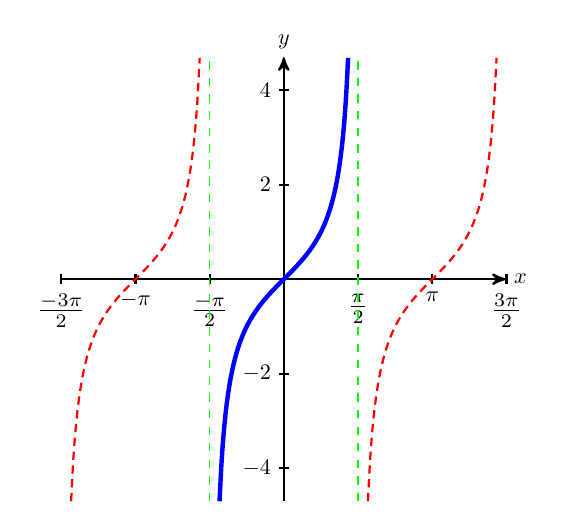
\begin{tikzpicture} [scale=.6]
\draw[black,thick,->,>=stealth'] (-3*pi/2,0)--(4.7,0) node[right, scale=.8] {$x$};
\draw[black,thick,->,>=stealth'] (0,-4.7)--(0,4.7) node[above, scale=.8] {$y$};
\foreach \y in {-4,-2,2,4} \draw[black,thick] (.1,\y)--++(-.2,0) node[left, scale=.8] {$\y$};
\draw[black,thick] (-3*pi/2,0.1)--++(0,-.2) node [below] {$\frac{-3\pi}{2} $};
\draw[black,thick] (-pi/2,0.1)--++(0,-.2) node [below] {$\frac{-\pi}{2} $};
\draw[black,thick] (-pi,0.1)--++(0,-.2) node [below, scale=.8] {$-\pi$};
\draw[black,thick] (pi/2,0.1)--++(0,-.2) node [below] {$\frac{\pi}{2} $};
\draw[black,thick] (pi,0.1)--++(0,-.2) node [below, scale=.8] {$\pi$};
\draw[black,thick] (3*pi/2,0.1)--++(0,-.2) node [below] {$\frac{3\pi}{2} $};
\draw[green, dashed] (-pi/2,-4.7)--++(0,9.4);
\draw[green, dashed] (pi/2,-4.7)--++(0,9.4);
\draw[samples=65,domain={-atan(4.7)*pi/180}:{atan(4.7)*pi/180},variable=\x, smooth, red, thick, densely dashed] plot (\x-pi,{tan(deg(\x))});
\draw[samples=65,domain={-atan(4.7)*pi/180}:{atan(4.7)*pi/180},variable=\x, smooth, red, thick, densely dashed] plot (\x+pi,{tan(deg(\x))});
\draw[samples=65,domain={-atan(4.7)*pi/180}:{atan(4.7)*pi/180},variable=\x, smooth, blue, ultra thick] plot (\x,{tan(deg(\x))});
\end{tikzpicture}
\newline

fig-8-2-10 inverse tangent

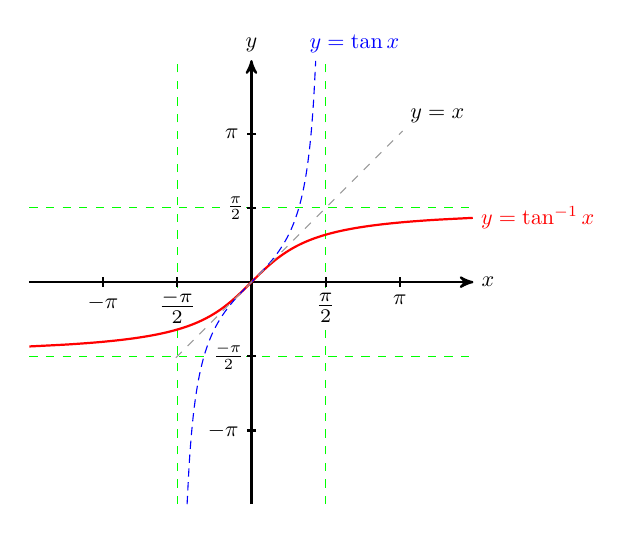
\begin{tikzpicture} [scale=0.6]
\draw[black,thick,->,>=stealth'] (-3*pi/2,0)--(4.7,0) node[right, scale=.8] {$x$};
\draw[black,thick,->,>=stealth'] (0,-4.7)--(0,4.7) node[above, scale=.8] {$y$};
\draw[green, dashed] (-4.7,pi/2)--++(9.4,0);
\draw[green, dashed] (-4.7,-pi/2)--++(9.4,0);
\draw[green, dashed] (-pi/2,-4.7)--++(0,9.4);
\draw[green, dashed] (pi/2,-4.7)--++(0,9.4);
\foreach \y in {pi} {
  \draw[black,thick] (.1,\y)--++(-.2,0) node[left, scale=.8] {$\pi$};
  \draw[black,thick] (.1,-\y)--++(-.2,0) node[left, scale=.8] {$-\pi$};
 };
  \draw[black,thick] (.1,-pi/2)--++(-.2,0) node[left, scale=.8, fill=white, inner sep = 1] {$\frac{-\pi}{2} $};
  \draw[black,thick] (.1,pi/2)--++(-.2,0) node[left, scale=.8, fill=white, inner sep = 1] {$\frac{\pi}{2} $};
\draw[black,thick] (-pi/2,0.1)--++(0,-.2) node [below, fill=white, inner sep = 1] {$\frac{-\pi}{2} $};
\draw[black,thick] (-pi,0.1)--++(0,-.2) node [below, scale=.8] {$-\pi$};
\draw[black,thick] (pi/2,0.1)--++(0,-.2) node [below, fill=white, inner sep = 1, yshift=-1] {$\frac{\pi}{2} $};
\draw[black,thick] (pi,0.1)--++(0,-.2) node [below, scale=.8] {$\pi$};
\draw[samples=65,domain={-atan(4.7)*pi/180}:{atan(4.7)*pi/180},variable=\x, smooth, red, thick] plot ({tan(deg(\x))},\x) node[right, scale=.8] {$y=\tan^{-1} x$};
\draw[samples=65,domain={-atan(4.7)*pi/180}:{atan(4.7)*pi/180},variable=\x, smooth, blue, densely dashed] plot (\x,{tan(deg(\x))}) node[above right, xshift=-5, scale=.8] {$y=\tan  x$};;
\draw[gray!80!white, dashed] (-1.6,-1.6)--(3.2,3.2) node[above right, scale=.8, text=black] {$y=x$};
\end{tikzpicture}
\newline

exam8-2-7 triangle
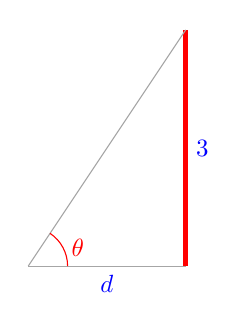
\begin{tikzpicture}
\coordinate (O) at (0,0);
\coordinate (A) at (2,0);
\coordinate (B) at (2,3);
\draw[red, ultra thick] (A)--(B) node[right, midway, scale=.9, text=blue] {3};
\draw[gray!70!white] (O)--(A) node[below, midway, text=blue, scale=.9] {$d$};
\draw[gray!70!white] (O)--(B) ;
\draw[red] (0.5,0) arc (0:atan(3/2): 0.5) node [right, midway, scale=.9] {$\theta$};
\end{tikzpicture}
\newline

exer8-2-7 triangle
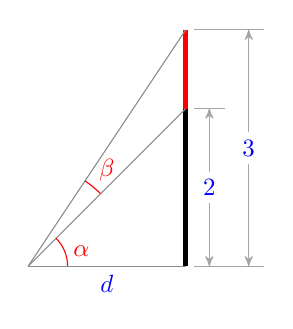
\begin{tikzpicture}
\coordinate (O) at (0,0);
\coordinate (A) at (2,0);
\coordinate (B) at (2,3);
\coordinate (C) at (2,2);
\draw[red, ultra thick] (A)--(B);
\draw[black, ultra thick] (A)--(C);
\draw[gray!90!white] (O)--(A) node[below, midway, text=blue, scale=.9] {$d$};
\draw[gray!90!white] (O)--(B) ;
\draw[gray!90!white] (O)--(C) ;
\draw[red] (0.5,0) arc (0:atan(2/2): 0.5) node [right, midway, scale=.9] {$\alpha$};
\draw[red] ({atan(3/2)}:1.3) arc (atan(3/2):atan(1): 1.3) node [above right, xshift=-1,yshift=-1, midway, scale=.9] {$\beta$};
\draw[gray!70!white] ((2.1,3)--++(0.9,0);
\draw[gray!70!white] ((2.1,2)--++(0.4,0);
\draw[gray!70!white] ((2.1,0)--++(0.9,0);

\draw[gray!70!white,<-,>=stealth'] ((2.3,2)--++(0, -.8);
\draw[gray!70!white,<-,>=stealth'] ((2.3,0)--++(0, .8);
\node[scale=.9, text=blue] at (2.3,1) {$2$};
\draw[gray!70!white,<-,>=stealth'] ((2.8,3)--++(0, -1.3);
\draw[gray!70!white,<-,>=stealth'] ((2.8,0)--++(0, 1.3);
\node[scale=.9, text=blue] at (2.8,1.5) {$3$};
\end{tikzpicture}
\newline

fig-8-2-11 unit circle

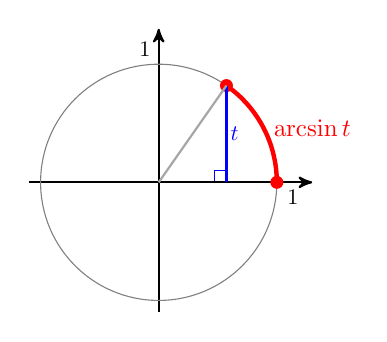
\begin{tikzpicture} [scale=1.5]
\def\th{55};
\coordinate (O) at (0,0);
\coordinate (A) at (1,0);
\coordinate (B) at ({\th}:1);
\coordinate (D) at ($ cos(\th)*(1,0)$);
\draw[blue] (D) rectangle ++(-.1,.1);
\draw[black,thick,->,>=stealth'] (-1.1,0)--(1.3,0) node[below left, xshift=-2, scale=.8] {1};
\draw[black,thick,->,>=stealth'] (0,-1.1)--(0,1.3) node[below left, yshift=-2, scale=.8] {1};
\draw[gray] (O) circle (1cm);
\draw[red,ultra thick] (A) arc(0:{\th}:1) node[right, midway, scale=.9] {$\arcsin t$};
\filldraw[red] (A) circle (.05cm);
\filldraw[red] (B) circle (.05cm);
\draw[blue,thick] (D)--(B) node[right, midway, scale=.8, inner sep=1.5] {$t$};
\draw[gray!70!white,thick] (O)--(B);
\end{tikzpicture}
\newline

ar8-2-1ans  linear function and inverse

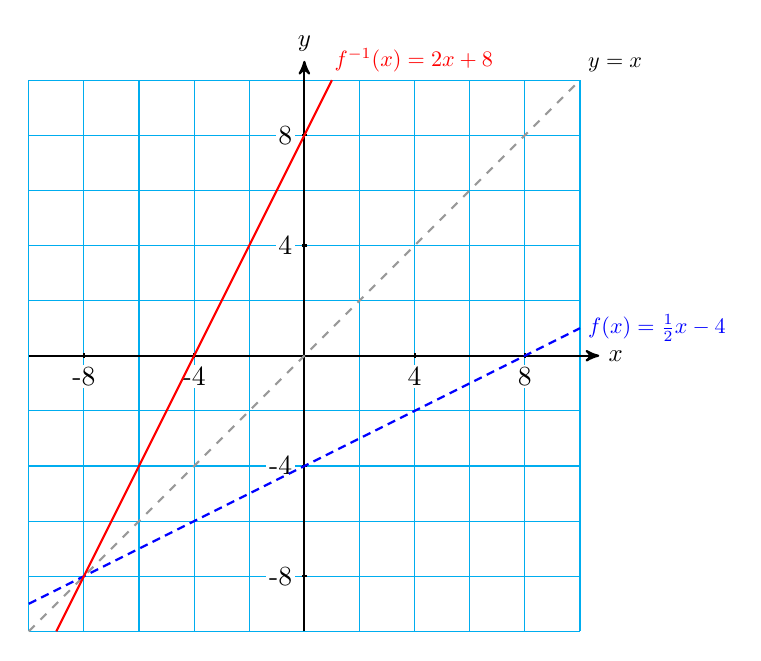
\begin{tikzpicture} [scale=0.35]
\draw[cyan] (-10,-10) grid[step=2] (10,10);
\draw[black,thick,->,>=stealth'] (-10,0)--(10.7,0) node[right, scale=.9] {$x$};
\draw[black,thick,->,>=stealth'] (0,-10)--(0,10.7) node[above, scale=.9] {$y$};
\foreach \x in {-8,-4,4,8} {
  \draw[black,thick] (\x,0.1)--++(0,-.2) node[below, yshift=-2, fill=white, inner sep=1] {\x};
  \draw[black,thick] (0.1,\x)--++(-.2,0) node[left, xshift=-2, fill=white, inner sep=1] {\x};
};
\draw[gray!80!, thick, dashed] (-10,-10)--(10,10) node[above right, text=black, scale=.8] {$y=x$};
\draw[blue, densely dashed,thick] (-10,-9)--(10,1) node[right, scale=.8] {$f(x)=\frac{1}{2}x-4$};
\draw[red, thick] (-9,-10)--(1,10) node[above right, xshift=-2, scale=.8] {$f^{-1}(x)=2x+8 $};
\end{tikzpicture}
\newline

ar8-2-2ans  linear function and inverse

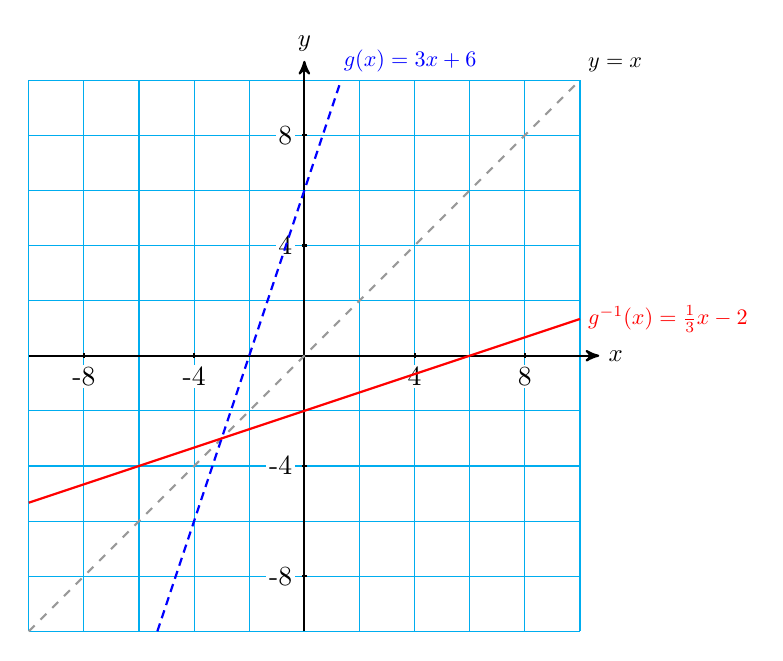
\begin{tikzpicture} [scale=0.35]
\draw[cyan] (-10,-10) grid[step=2] (10,10);
\draw[black,thick,->,>=stealth'] (-10,0)--(10.7,0) node[right, scale=.9] {$x$};
\draw[black,thick,->,>=stealth'] (0,-10)--(0,10.7) node[above, scale=.9] {$y$};
\foreach \x in {-8,-4,4,8} {
  \draw[black,thick] (\x,0.1)--++(0,-.2) node[below, yshift=-2, fill=white, inner sep=1] {\x};
  \draw[black,thick] (0.1,\x)--++(-.2,0) node[left, xshift=-2, fill=white, inner sep=1] {\x};
};
\draw[gray!80!, thick, dashed] (-10,-10)--(10,10) node[above right, text=black, scale=.8] {$y=x$};
\draw[blue, densely dashed,thick] (-16/3,-10)--(4/3,10) node[above right, xshift=-2, scale=.8] {$g(x)=3x+6$};
\draw[red, thick] (-10,-16/3)--(10,4/3) node[ right, scale=.8] {$g^{-1}(x)=\frac{1}{3} x-2 $};
\end{tikzpicture}
\newline

ar8-2-3ans  transformed reciprocal function

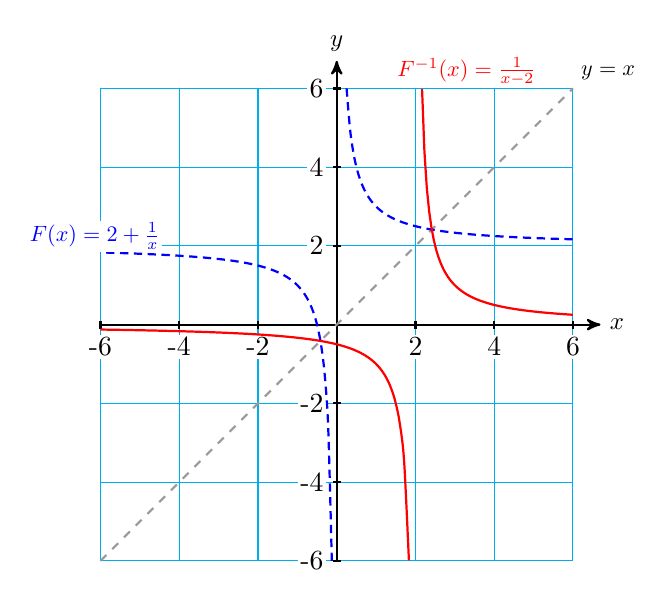
\begin{tikzpicture} [scale=0.5]
\draw[cyan] (-6,-6) grid[step=2] (6,6);
\draw[black,thick,->,>=stealth'] (-6,0)--(6.7,0) node[right, scale=.9] {$x$};
\draw[black,thick,->,>=stealth'] (0,-6)--(0,6.7) node[above, scale=.9] {$y$};
\foreach \x in {-6,-4,-2,2,4,6} {
  \draw[black,thick] (\x,0.1)--++(0,-.2) node[below, yshift=-2, fill=white, inner sep=1] {\x};
  \draw[black,thick] (0.1,\x)--++(-.2,0) node[left, xshift=-2, fill=white, inner sep=1] {\x};
};
\draw[gray!80!, thick, dashed] (-6,-6)--(6,6) node[above right, text=black, scale=.8] {$y=x$};
\draw[samples=65,domain=-1/8:-6, variable=\x, smooth, blue, densely dashed,thick] plot (\x,{ 2+1/\x}) node[above , xshift=-2, scale=.8, fill=white, inner sep=1] {$F(x)=2+\frac{1}{x} $};
\draw[samples=65,domain=1/4:6, variable=\x, smooth, blue, densely dashed,thick] plot (\x,{ 2+1/\x});
\draw[samples=65,domain=-6:11/6, variable=\x, smooth ,red, thick] plot (\x,{ 1/(\x-2)});
\draw[samples=65,domain=6:13/6, variable=\x ,red, thick] plot (\x,{ 1/(\x-2)}) node[above right, xshift=-10, scale=.8, inner sep=1]  {$F^{-1}(x)=\frac{1}{ x-2} $};
\end{tikzpicture}
\newline

ar8-2-4ans  transformed reciprocal function

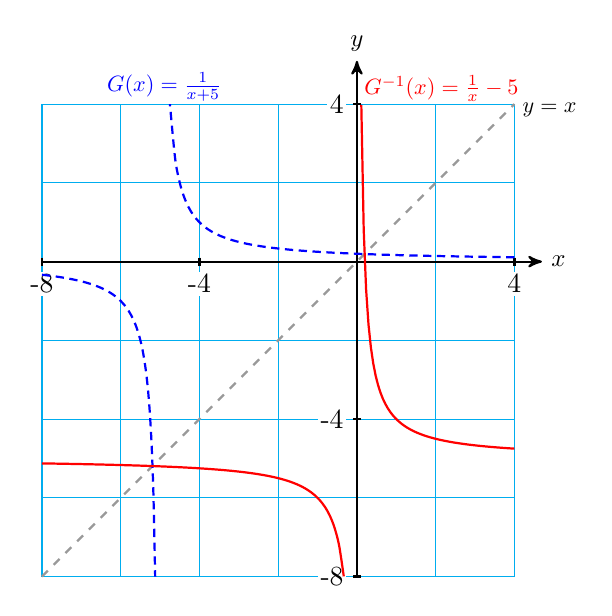
\begin{tikzpicture} [scale=0.5]
\draw[cyan] (-8,-8) grid[step=2] (4,4);
\draw[black,thick,->,>=stealth'] (-8,0)--(4.7,0) node[right, scale=.9] {$x$};
\draw[black,thick,->,>=stealth'] (0,-8)--(0,5.1) node[above, scale=.9] {$y$};
\foreach \x in {-8,-4,4} {
  \draw[black,thick] (\x,0.1)--++(0,-.2) node[below, yshift=-2, fill=white, inner sep=1] {\x};
  \draw[black,thick] (0.1,\x)--++(-.2,0) node[left, xshift=-2, fill=white, inner sep=1] {\x};
};
\draw[gray!80!, thick, dashed] (-8,-8)--(4,4) node[ right, yshift=-2, text=black, scale=.8] {$y=x$};
\draw[samples=65,domain=4:-19/4, variable=\x, smooth, blue, densely dashed,thick] plot (\x,{ 1/(\x+5)}) node[above , xshift=-2, scale=.8, fill=white, inner sep=1] {$G(x)=\frac{1}{x+5} $};
\draw[samples=65,domain=-8:-41/8, variable=\x, smooth, blue, densely dashed,thick] plot (\x,{ 1/(\x+5)});
\draw[samples=65,domain=-8:-1/3, variable=\x, smooth ,red, thick] plot (\x,{ 1/(\x)-5});
\draw[samples=65,domain=4:1/9, variable=\x ,red, thick] plot (\x,{ 1/(\x)-5}) node[above right, xshift=0, scale=.8, inner sep=1]  {$G^{-1}(x)=\frac{1}{ x}-5 $};
\end{tikzpicture}
\newline

ar8-2-5ans  transformed square root

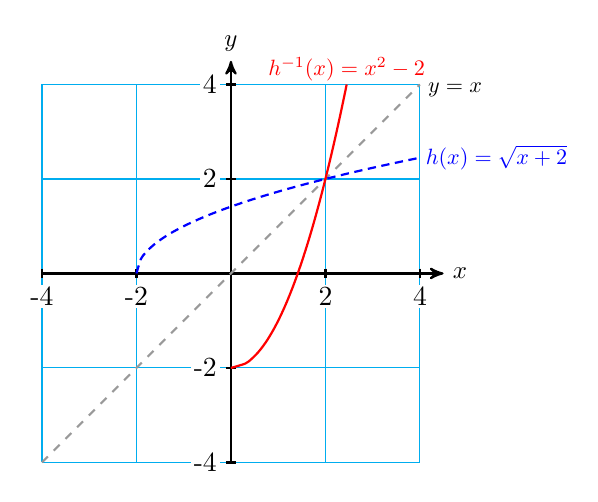
\begin{tikzpicture} [scale=0.6]
\draw[cyan] (-4,-4) grid[step=2] (4,4);
\draw[black,thick,->,>=stealth'] (-4,0)--(4.5,0) node[right, scale=.9] {$x$};
\draw[black,thick,->,>=stealth'] (0,-4)--(0,4.5) node[above, scale=.9] {$y$};
\foreach \x in {-2,2,-4,4} {
  \draw[black,thick] (\x,0.1)--++(0,-.2) node[below, yshift=-2, fill=white, inner sep=1] {\x};
  \draw[black,thick] (0.1,\x)--++(-.2,0) node[left, xshift=-2, fill=white, inner sep=1] {\x};
};
\draw[gray!80!, thick, dashed] (-4,-4)--(4,4) node[ right, yshift=-2, text=black, scale=.8] {$y=x$};
\draw[samples=65,domain=-2:4, variable=\x, smooth, blue, densely dashed,thick] plot (\x,{ sqrt(\x+2) }) node[right, xshift=1,  scale=.8, fill=white, inner sep=1] {$h(x)=\sqrt{x+2} $};
\draw[samples=65,domain=-2:4, variable=\x, smooth ,red, thick] plot ({ sqrt(\x+2) },\x) node[above , xshift=0, scale=.8, inner sep=1]  {$h^{-1}(x)=x^2 -2 $};
\end{tikzpicture}
\newline

ar8-2-6ans  transformed cube root

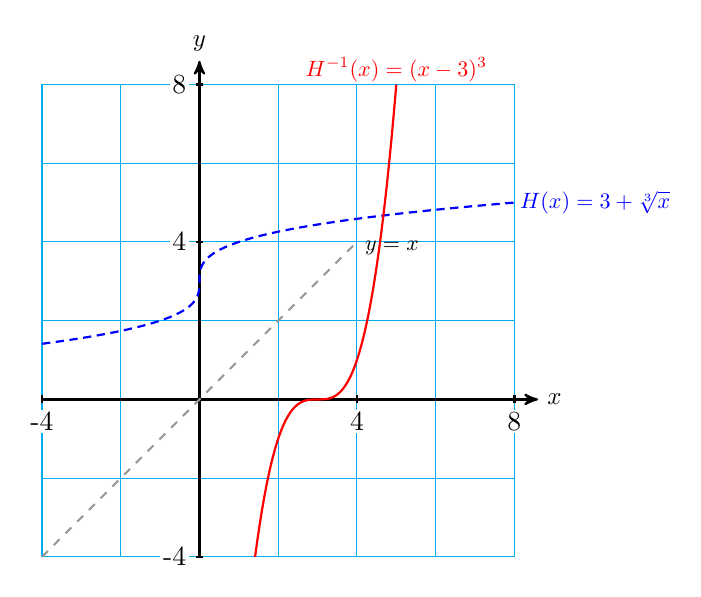
\begin{tikzpicture} [scale=0.5]
\draw[cyan] (-4,-4) grid[step=2] (8,8);
\draw[black,thick,->,>=stealth'] (-4,0)--(8.6,0) node[right, scale=.9] {$x$};
\draw[black,thick,->,>=stealth'] (0,-4)--(0,8.6) node[above, scale=.9] {$y$};
\foreach \x in {8,-4,4} {
  \draw[black,thick] (\x,0.1)--++(0,-.2) node[below, yshift=-2, fill=white, inner sep=1] {\x};
  \draw[black,thick] (0.1,\x)--++(-.2,0) node[left, xshift=-2, fill=white, inner sep=1] {\x};
};
\draw[gray!80!, thick, dashed] (-4,-4)--(4,4) node[ right, yshift=-2, text=black, scale=.8] {$y=x$};
\draw[samples=65,domain={3-4^(1/3)}:5, variable=\x, smooth, blue, densely dashed,thick] plot ({(\x-3)^3},\x) node[right, xshift=1,  scale=.8, fill=white, inner sep=1] {$H(x)=3+\sqrt[3]{x} $};
\draw[samples=65,domain={3-4^(1/3)}:5, variable=\x, smooth ,red, thick] plot (\x,{ (\x-3)^3 }) node[above , xshift=0, scale=.8, inner sep=1]  {$H^{-1}(x)=(x-3)^3 $};
\end{tikzpicture}
\newline


sq8-2-5 triangle

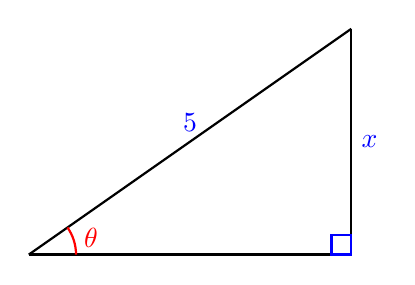
\begin{tikzpicture}
\coordinate (O) at (0,0);
\def\th{35};
\coordinate (A) at (\th:5);
\coordinate (B) at ($ 5*cos(\th)*(1,0) $);
\draw[black,thick] (O)--(A) node[above, midway, text=blue]{$5$};
\draw[black,thick] (B)--(A) node[right, midway, text=blue]{$x$};
\draw[black,thick] (O)--(B);
\draw[blue,thick] (B) rectangle ++(-.25,.25);
\draw[red, thick] (0.6,0) arc(0:{\th}:0.6) node[right, yshift=1, midway] {$\theta$};
\end{tikzpicture}
\newline



sq8-2-6 triangle

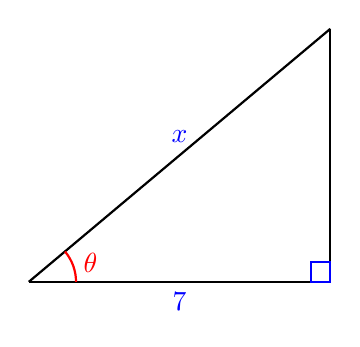
\begin{tikzpicture}
\coordinate (O) at (0,0);
\def\th{40};
\coordinate (A) at (\th:5);
\coordinate (B) at ($ 5*cos(\th)*(1,0) $);
\draw[black,thick] (O)--(A) node[above, yshift=1, midway, text=blue]{$x$};
\draw[black,thick] (B)--(A);
\draw[black,thick] (O)--(B) node[below, midway, text=blue]{$7$};
\draw[blue,thick] (B) rectangle ++(-.25,.25);
\draw[red, thick] (0.6,0) arc(0:{\th}:0.6) node[right, yshift=1, midway] {$\theta$};
\end{tikzpicture}
\newline


hp8-2-1 sine plus linear

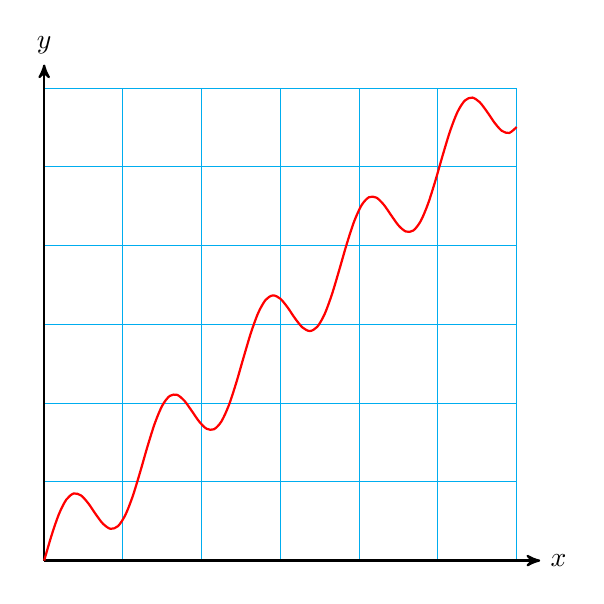
\begin{tikzpicture}
\draw [cyan] (0,0) grid (6,6);
\draw[black,thick,->,>=stealth'] (0,0)--(6.3,0) node[right]{$x$};
\draw[black,thick,->,>=stealth'] (0,0)--(0,6.3) node[above]{$y$};
\draw[samples=65,domain=0:6, variable=\x, smooth, red, thick] plot (\x, {sin(5*deg(\x))/2 + \x});
\end{tikzpicture}
\newline


hp8-2-2 y=8-12/(x+2)

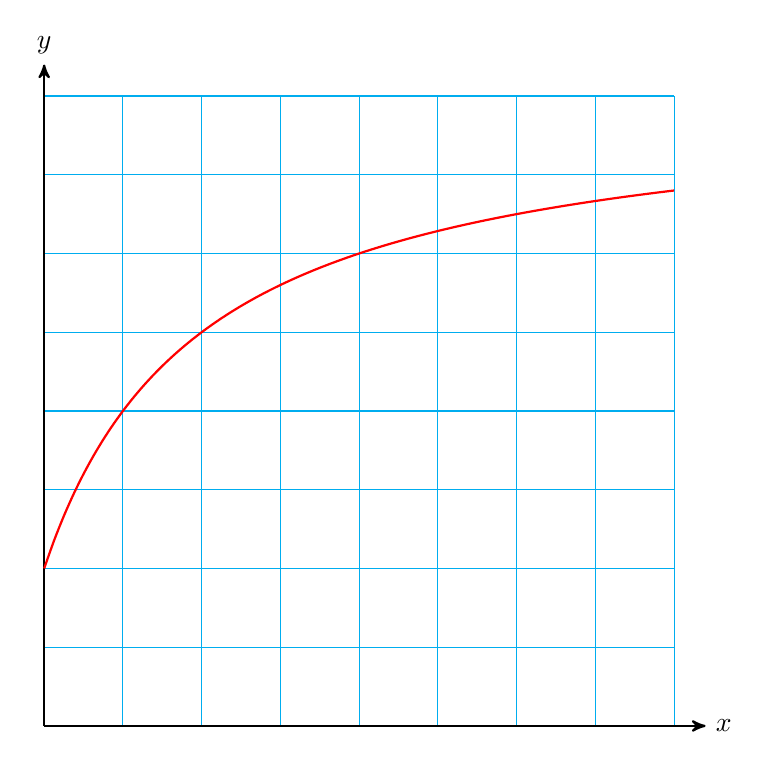
\begin{tikzpicture}
\draw [cyan] (0,0) grid (8,8);
\draw[black,thick,->,>=stealth'] (0,0)--(8.4,0) node[right]{$x$};
\draw[black,thick,->,>=stealth'] (0,0)--(0,8.4) node[above]{$y$};
\draw[samples=65,domain=0:8, variable=\x, smooth, red, thick] plot (\x, { 8-12/(\x+2) });
\end{tikzpicture}
\newline


hp8-2-3 transformed cubic

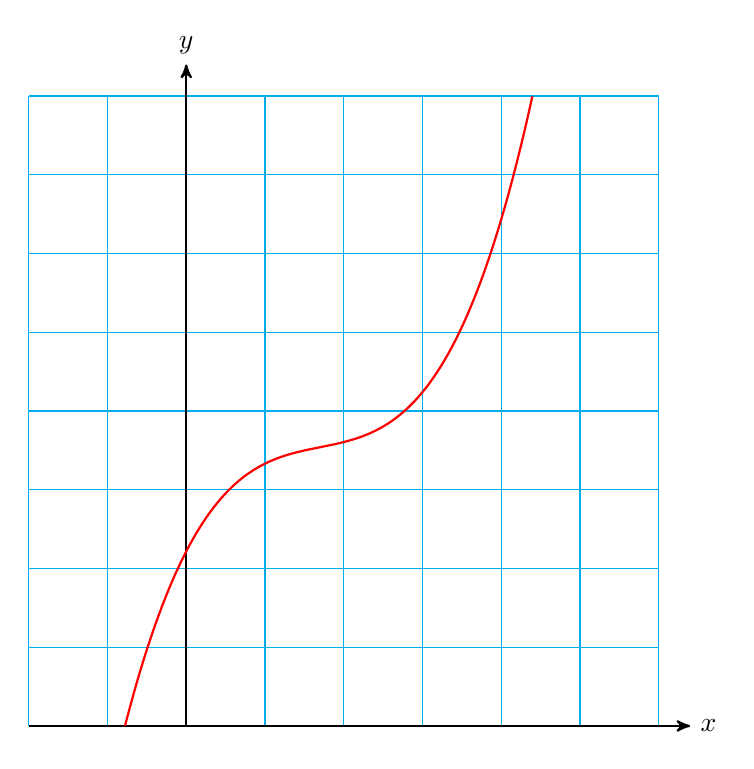
\begin{tikzpicture}
\draw [cyan] (-2,0) grid (6,8);
\draw[black,thick,->,>=stealth'] (-2,0)--(6.4,0) node[right]{$x$};
\draw[black,thick,->,>=stealth'] (0,0)--(0,8.4) node[above]{$y$};
\draw[samples=65,domain=-.778:4.396, variable=\x, smooth, red, thick] plot (\x, { .2*(\x-1.7)^3+3.2 +\x/5});
\end{tikzpicture}
\newline


hp8-2-4 quartic

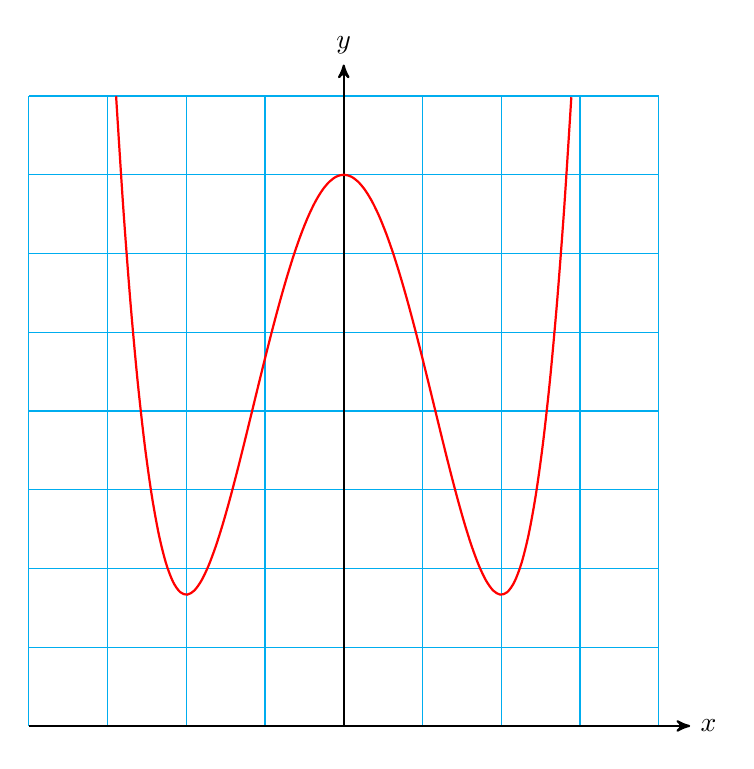
\begin{tikzpicture}
\draw [cyan] (-4,0) grid (4,8);
\draw[black,thick,->,>=stealth'] (-4,0)--(4.4,0) node[right]{$x$};
\draw[black,thick,->,>=stealth'] (0,0)--(0,8.4) node[above]{$y$};
\draw[samples=65,domain=-2.891:2.891, variable=\x, smooth, red, thick] plot (\x, { (\x)^2*((\x)^2-8)/3+7 });
\end{tikzpicture}
\newline

hp8-2-5ans sin2x - cos x

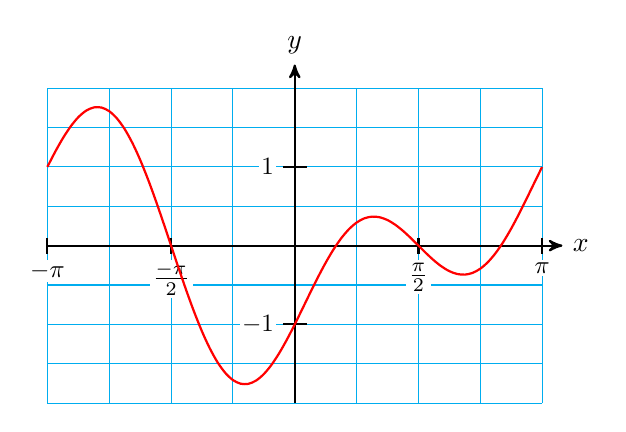
\begin{tikzpicture}
\draw [cyan] (-pi,-2) grid[xstep=pi/4, ystep=1/2] (pi,2);
\draw[black,thick,->,>=stealth'] (-pi,0)--(3.4,0) node[right]{$x$};
\draw[black,thick,->,>=stealth'] (0,-2)--(0,2.3) node[above]{$y$};
\foreach \y in {-1,1} \draw[black,thick] (.15,\y)--++(-.3,0) node[left, xshift=-2, fill=white, inner sep=1, scale=.9] {$\y$};
\draw[black,thick] (-pi,.1)--++(0,-.2) node[below, yshift=-2, fill=white, inner sep=1, scale=.9] {$-\pi$};
\draw[black,thick] (-pi/2,.1)--++(0,-.2) node[below, yshift=-2, fill=white, inner sep=1] {$\frac{-\pi}{2} $};
\draw[black,thick] (pi/2,.1)--++(0,-.2) node[below, yshift=-2, fill=white, inner sep=1] {$\frac{\pi}{2} $};
\draw[black,thick] (pi,.1)--++(0,-.2) node[below, yshift=-2, fill=white, inner sep=1, scale=.9] {$\pi$};
\draw[samples=65,domain=-pi:pi, variable=\x, smooth, red, thick] plot (\x, { sin(deg(2*\x)) - cos(deg(\x)) });
\end{tikzpicture}
\newline

hp8-2-7ans $ \sqrt{25=x^2}$

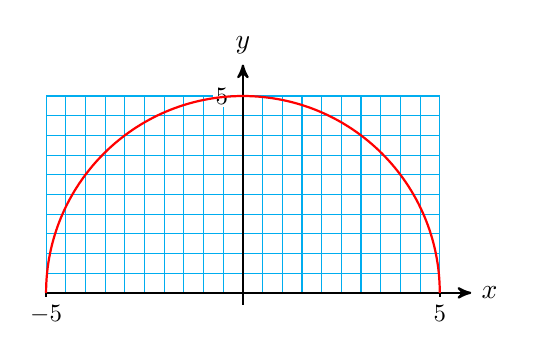
\begin{tikzpicture} [scale=.5]
\draw [cyan] (-5,0) grid[step=1/2] (5,5);
\draw[black,thick,->,>=stealth'] (-5,0)--(5.8,0) node[right]{$x$};
\draw[black,thick,->,>=stealth'] (0,-.3)--(0,5.8) node[above]{$y$};
\draw[black,thick] (.15,5)--++(-.3,0) node[left, xshift=-2, fill=white, inner sep=1, scale=.9] {$5$};
\foreach \x in {-5,5} \draw[black,thick] (\x,.1)--++(0,-.2) node[below, yshift=-2, fill=white, inner sep=1, scale=.9] {$\x$};
\draw[red, thick] (5,0) arc (0:180:5);
\end{tikzpicture}
\newline

hp8-2-21ans triangle

\begin{tikzpicture} 
\draw[blue] (2,0) rectangle ++(-.25,.25);
\draw[black,thick] (0,0) -- (2,0) node[below, midway, xshift=2, text=blue] {500 yd};
\draw[gray,thick] (2,0) --++(0,3) node[right, midway, text=blue] {$h$};
\draw[gray,thick] (0,0)--(2,3);
\draw[red,thick] (0.3,0) arc(0:atan(3/2):0.3) node[right, midway, yshift=1] {$\theta$};
\end{tikzpicture}
\newline

hp8-2-23ans triangle

\begin{tikzpicture} 
\draw[blue] (0,0) rectangle ++(.25,-.25);
\draw[black,thick] (0,0) -- (2,0) node[above, midway, xshift=2, text=blue] {50 ft};
\draw[gray,thick] (0,0) --++(0,-3.5) node[left, midway, text=blue] {$d$};
\draw[gray,thick] (0,-3.5)--(2,0);
\draw[red,thick] (-90:3.) arc(90:atan(3.5/2):0.5) node[above, midway, xshift=2] {$\theta$};
\end{tikzpicture}
\newline

hp8-2-25ans triangle [scale=.8]

\begin{tikzpicture} 
\draw[blue] (5,0) rectangle ++(-.25,.25);
\draw[black,thick] (0,0) -- (5,0) node[below, midway, xshift=2, text=blue] {$x$};
\draw[gray,thick] (5,0) --++(0,1) node[right, midway, text=blue] {1 m};
\draw[red, ultra thick] (5,1) --++(0,4) node[right, midway, text=blue] {4 m};
\draw[gray,thick] (5,1)--(0,0)--(5,5);
\draw[red,thick] (2,0) arc(0:atan(1/5):2) node[right, midway] {$\alpha$};
\draw[red,thick] ({atan(1/5)}:1) arc({atan(1/5)}:45:1) node[above right, midway, yshift=-2] {$\beta$};
\end{tikzpicture}
\newline

hp8-2-45 grid

\begin{tikzpicture}
\draw[cyan] (-2,-pi) grid[xstep=1/2, ystep=pi/6] (2,pi);
\draw[black,thick,->,>=stealth'] (0,-pi)--(0,3.35) node[above, scale=.8]{$y$};
\draw[black,thick,->,>=stealth'] (-2,0)--(2.3,0) node[right, scale=.8]{$x$};
\foreach \x in {-2,-1,1,2} \draw[black,thick](\x,.1)--++(0,-.2) node[below, fill=white, inner sep=1, yshift=-2, scale=.8]{\x};
\end{tikzpicture}
\newline

hp8-2-45ans arccos

\begin{tikzpicture}
\draw[cyan] (-2,0) grid[xstep=1/2, ystep=pi/6] (2,pi);
\draw[black,thick,->,>=stealth'] (0,-.2)--(0,3.35) node[above, scale=.8]{$y$};
\draw[black,thick] (.1,pi)--++(-.2,0) node [left, xshift=-2, fill=white, inner sep=1, scale=.8] {$\pi$};
\draw[black,thick] (.1,pi/2)--++(-.2,0) node [left, xshift=-2, fill=white, inner sep=1] {$\frac{\pi}{2}$};
\draw[black,thick,->,>=stealth'] (-2,0)--(2.3,0) node[right, scale=.8]{$x$};
\foreach \x in {-2,-1,1,2} \draw[black,thick](\x,.1)--++(0,-.2) node[below, fill=white, inner sep=1, yshift=-2, scale=.8]{\x};
\draw[samples=65, variable=\x,domain=0:pi, smooth, red, thick] plot ({cos(deg(\x))},\x);
\end{tikzpicture}
\newline

hp8-2-47 grid

\begin{tikzpicture}
\draw[cyan] (-4,-pi) grid[xstep=1/2, ystep=pi/6] (4,pi);
\draw[black,thick,->,>=stealth'] (0,-pi)--(0,3.35) node[above]{$y$};
\draw[black,thick,->,>=stealth'] (-4,0)--(4.3,0) node[right]{$x$};
\foreach \x in {-2,2,-4,4} \draw[black,thick](\x,.1)--++(0,-.2) node[below, fill=white, inner sep=1, yshift=-2]{$\x$};
\end{tikzpicture}
\newline

hp8-2-47ans arctan

\begin{tikzpicture}
\draw[cyan] (-4,-pi/2) grid[xstep=1/2, ystep=pi/6] (4,pi/2);
\draw[black,thick,->,>=stealth'] (0,-pi/2)--(0,1.8) node[above]{$y$};
\draw[black,thick,->,>=stealth'] (-4,0)--(4.3,0) node[right]{$x$};
\foreach \x in {-2,2,-4,4} \draw[black,thick](\x,.1)--++(0,-.2) node[below, fill=white, inner sep=1, yshift=-2]{$\x$};
\draw[black,thick] (.1,pi/2)--++(-.2,0) node [left, xshift=-2, fill=white, inner sep=1] {$\frac{\pi}{2}$};
\draw[black,thick] (.1,-pi/2)--++(-.2,0) node [left, xshift=-2, fill=white, inner sep=1] {$\frac{-\pi}{2}$};
\draw[samples=65, variable=\x,domain=-4:4, smooth, red, thick] plot (\x,{atan(\x)*pi/180});
\end{tikzpicture}
\newline

hp8-2-49ans transformed arccos

\begin{tikzpicture} [xscale=1.2,yscale=.65]
\draw[cyan] (-1,0) grid[xstep=1/2, ystep=pi/3] (1,2*pi);
\draw[black,thick,->,>=stealth'] (0,-.2)--(0,6.4) node[above, xscale=.8]{$y$};
\draw[black,thick,->,>=stealth'] (-1,0)--(1.2,0) node[right, xscale=.8]{$x$};
\foreach \x in {-1,1} \draw[black,thick](\x,.2)--++(0,-.4) node[below, fill=white, inner sep=1, yshift=-2, xscale=.8]{$\x$};
\draw[black,thick] (.1,pi)--++(-.2,0) node [left, xshift=-2, fill=white, inner sep=1, xscale=.8] {$\pi$};
\draw[black,thick] (.1,2*pi)--++(-.2,0) node [left, xshift=-2, fill=white, inner sep=1, xscale=.8] {$2\pi$};
\draw[samples=65, variable=\x,domain=1:-1, smooth, red, thick] plot (\x,{acos(\x)*pi/180}) node[left, text=red, scale=.8] {$y=\cos^{-1}x$} ;
\draw[samples=65, variable=\x,domain=-1/2:1/2, smooth, green, thick] plot (\x,{acos(2*\x)*pi/180});
\draw[gray,<-,>=stealth'] (.45,-.1)--++(-.2,-.3)  node[below, xshift=-4, yshift=2, text=green!80!black, scale=.8] {$y=\cos^{-1}2x$}; 
\draw[samples=65, variable=\x,domain=1:-1, smooth, blue, thick] plot (\x,{2*acos(\x)*pi/180}) node[left, text=blue, scale=.9] {$y=2\cos^{-1}x$} ;
\end{tikzpicture}
\newline


hp8-2-73 unit circle

\begin{tikzpicture} [scale=1.5]
\def\th{55};
\coordinate (A) at ({\th}:1);
\coordinate (B) at ($ cos(\th) *(1,0) $);
\draw[blue] (B) rectangle ++(-.15,.15);
\filldraw[cyan!50!white] (0,0)--(A) arc({\th}:90:1)--(0,0);
\draw[black,thick,->,>=stealth'] (-1.2,0)--(1.3,0) node[below left, xshift = -2, scale=.9] {1};
\draw[black,thick,->,>=stealth'] (0,-1.2)--(0,1.3) node[below left, scale=.9] {1};
\draw[black,thick] (0,0) circle (1cm);
\draw[red,thick] ({\th}:0.3) arc({\th}:90:0.3) node[above right,scale=.9] {$\theta$};
\draw[gray,thick] (A)--(B) node[below, text=black, scale=.9] {$t$};
\draw[gray,thick] (A)--(0,0);
\end{tikzpicture}
\newline


hp8-2-73 unit circle

\begin{tikzpicture} [scale=1.5]
\def\th{55};
\coordinate (A) at ({\th}:1);
\coordinate (B) at ($ cos(\th) *(1,0) $);
\filldraw[cyan!50!white] (0,0)--(A)--(B) --(0,0);
\draw[blue] (B) rectangle ++(-.15,.15);
\draw[black,thick,->,>=stealth'] (-1.2,0)--(1.3,0) node[below left, xshift = -2, scale=.9] {1};
\draw[black,thick,->,>=stealth'] (0,-1.2)--(0,1.3) node[below left, scale=.9] {1};
\draw[black,thick] (0,0) circle (1cm);
\draw[red,thick] ({\th}:0.3) arc({\th}:90:0.3) node[above right,scale=.9] {$\theta$};
\draw[gray,thick] (A)--(B) node[below, text=black, scale=.9] {$t$};
\draw[gray,thick] (A)--(0,0);
\end{tikzpicture}
\newline











\end{document}
